\chapter{Sprint 1:  User and Submitted File Management}
\newpage
\begin{center}
    \centering
    \LARGE\textbf{Introduction} 
     \vspace{1cm} \\
   \raggedright
\end{center}
\addcontentsline{toc}{section}{Introduction}
In the previous chapter, we have identified all the different functional requirements in relation to our project. We have then broken down the project to plan the work phases in return. This chapter deals with the first sprint of our project, "User and Submitted File Management."
It is important to mention that every user story will go through all four stages of the Scrum process, functional specification, design, coding, and testing.
\section{Functional Specification}
At the beginning of each stage of a sprint, functional specification is carried out by means of a use case diagram to provide an overview of the system as well as to specify the various interactions between the system and the users.
\subsection{Sprint Backlog}
This refers to the set of features and tasks identified by the Scrum team from the product backlog, which will be completed during this sprint.

\renewcommand{\arraystretch}{1.2}
\setlength{\tabcolsep}{6pt}

\begin{longtable}
{|>{\centering\arraybackslash}p{0.7cm}%
 |>{\raggedright\arraybackslash}p{2.5cm}%
 |>{\raggedright\arraybackslash}p{3.2cm}%
 |>{\centering\arraybackslash}p{1.2cm}%
 |>{\raggedright\arraybackslash}p{5.3cm}|}
\hline
\textbf{Id} & \textbf{User Story} & \textbf{User Story Description} & \textbf{Task Id} & \textbf{Task} \\
\hline
\endfirsthead
\hline
1 & Authenticate & As a system user, I want to authenticate so that I can access features. & 1.1 & Create use case, system sequence, detailed sequence, and class diagrams for "Authenticate". \\
\cline{4-5}
& & & 1.2 & Implement the "Authenticate" use case. \\
\cline{4-5}
& & & 1.3 & Test the "Authenticate" use case. \\
\hline
2 & Submit a service request & As an insured user, I want to submit a service request to receive support. & 2.1 & Create diagrams for "Submit a service request". \\
\cline{4-5}
& & & 2.2 & Implement the service request form. \\
\cline{4-5}
& & & 2.3 & Test the service request submission. \\
\hline
3 & Manage my profile & As an insured user, I want to manage my profile to update my info. & 3.1 & Create diagrams for "Manage my profile". \\
\cline{4-5}
& & & 3.2 & Implement profile update feature. \\
\cline{4-5}
& & & 3.3 & Test profile management. \\
\hline
4 & Review submissions & As a coordinator, I want to review submissions to validate requests. & 4.1 & Create diagrams for "Review submissions". \\
\cline{4-5}
& & & 4.2 & Implement review interface. \\
\cline{4-5}
& & & 4.3 & Test the review process. \\
\hline
5 & Manage coordinator profile & As a coordinator, I want to manage my profile. & 5.1 & Create diagrams for "Manage coordinator profile". \\
\cline{4-5}
& & & 5.2 & Implement profile management. \\
\cline{4-5}
& & & 5.3 & Test profile functionality. \\
\hline
6 & Manage submission coordinators & As a central agent, I want to manage submission coordinators. & 6.1 & Create diagrams for "Manage submission coordinators". \\
\cline{4-5}
& & & 6.2 & Implement add/edit/delete functions. \\
\cline{4-5}
& & & 6.3 & Test coordinator management. \\
\hline
7 & Review Escalated submissions & As a central agent, I want to review submissions Escalated to central. & 7.1 & Create diagrams for "Review central submissions". \\
\cline{4-5}
& & & 7.2 & Implement review interface. \\
\cline{4-5}
& & & 7.3 & Test review functionality. \\
\hline
8 & Manage dynamic forms & As a manager, I want to manage dynamic forms used in submissions. & 8.1 & Create diagrams for "Manage dynamic forms". \\
\cline{4-5}
& & & 8.2 & Implement form creation/editing. \\
\cline{4-5}
& & & 8.3 & Test form management. \\
\hline
9 & Manage stakeholders & As a manager, I want to manage internal stakeholders. & 9.1 & Create diagrams for "Manage internal stakeholders". \\
\cline{4-5}
& & & 9.2 & Implement stakeholder management. \\
\cline{4-5}
& & & 9.3 & Test stakeholder management. \\
\hline
\caption{Product Backlog of Sprint 1.}
\end{longtable}
\clearpage
\section {Use Case Diagram of the First Sprint} 
\subsection{Classification of Use Cases by Actor}
This table presents a general classification of functionalities by actor.
\begin{figure}[h]
    \centering
    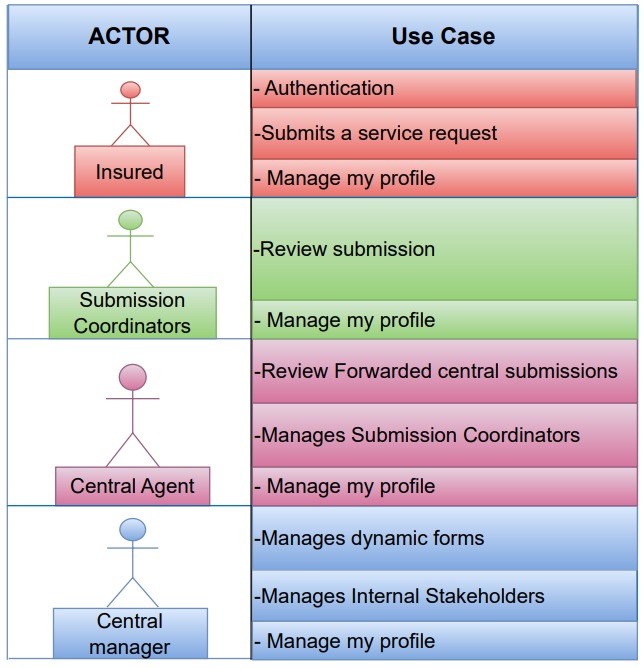
\includegraphics[width=1\textwidth]{figures/use case par acteur.png}
    \caption{Use Case Diagram by Actor.}
\end{figure}
\clearpage
\subsection{Diagramme de cas d’utilisation du premier sprint}
Le diagramme de cas d’utilisation initiale de premier sprint est présenté dans la figure suivante :
\begin{figure}[h]
    \centering
    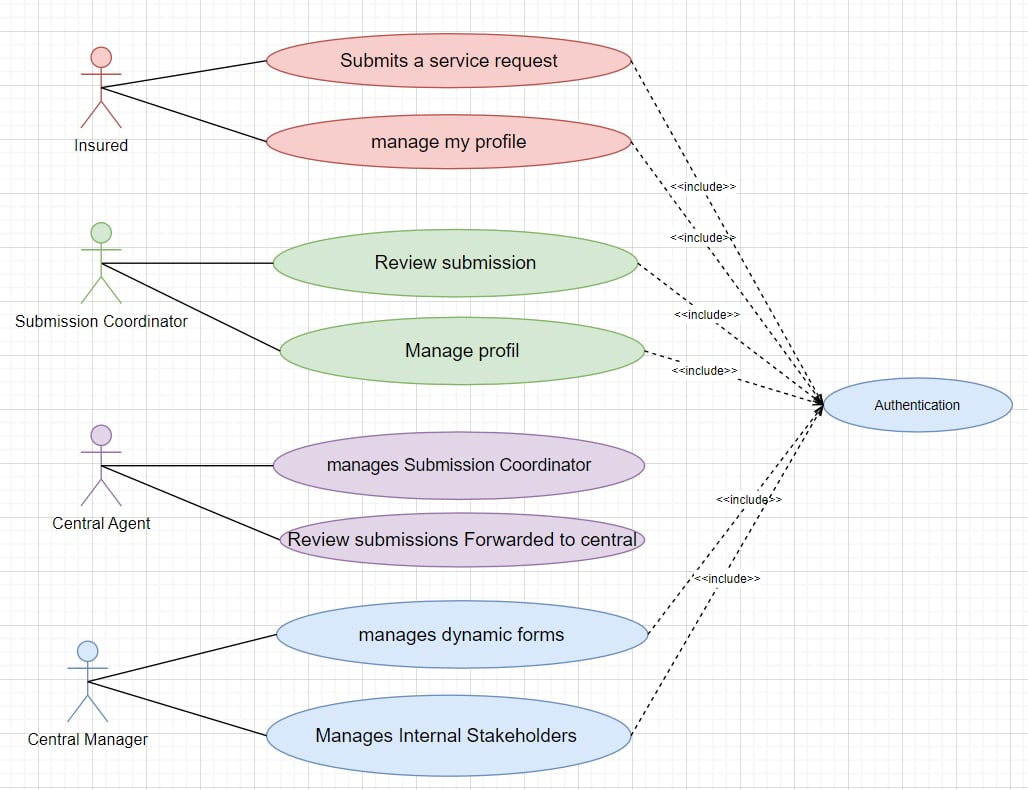
\includegraphics[width=1\textwidth]{figures/sprint1 use case.jpg}
    \caption{Use Case Diagram by Actor.}
\end{figure}
\clearpage
\subsection{Interface Prototyping}
This section aims to illustrate some prototypes of the interfaces developed during this sprint, showcasing the necessary features and interactions with our platform.
\begin{itemize}
    \item Authentication Interface Prototype
    \begin{figure}[h]
    \centering
    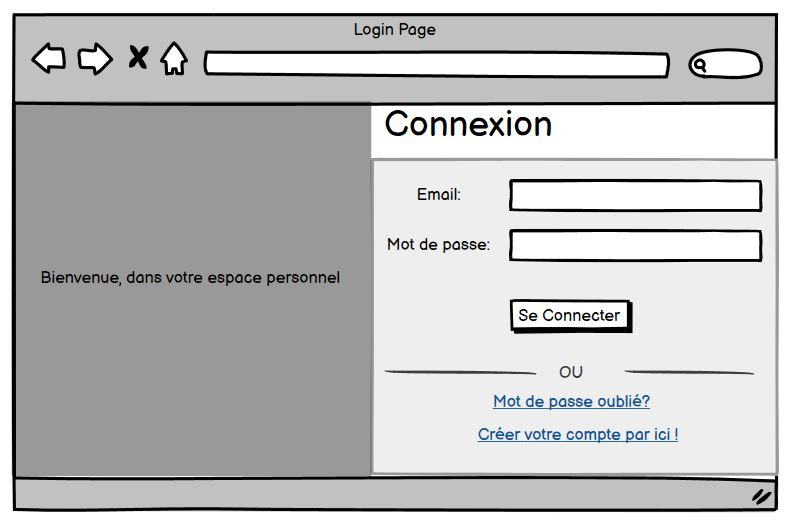
\includegraphics[width=0.9\textwidth]{figures/login.JPG}  % Replace with your image file
    \caption{Prototype of Login Page.}
\end{figure}\
\begin{figure}[h]
    \centering
    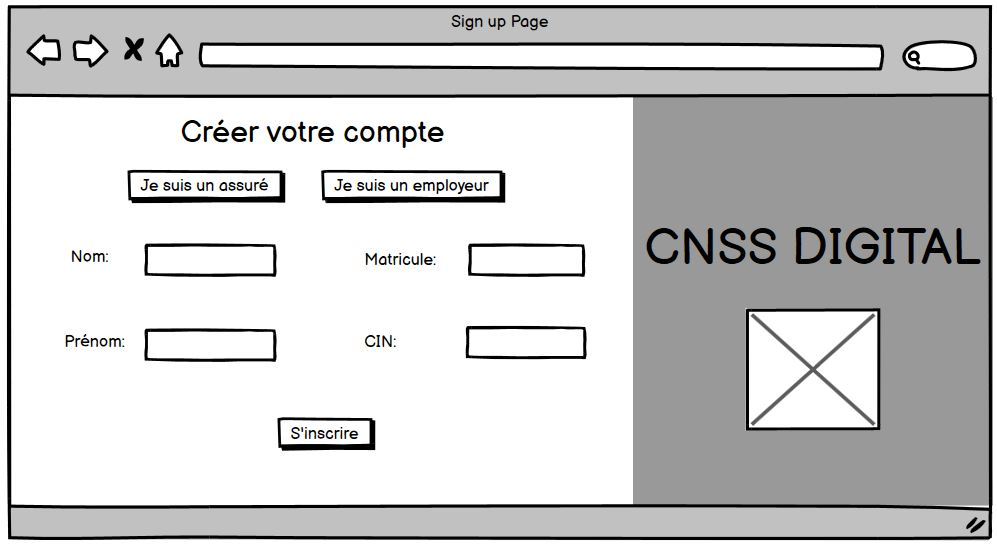
\includegraphics[width=0.9\textwidth]{figures/signup.JPG}  % Replace with your image file
    \caption{Prototype of Sign-up Page.}
\end{figure}\
\end{itemize}
\clearpage
\begin{itemize}
    \item Submission of a service request prototype
\begin{figure}[h!]
    \centering
    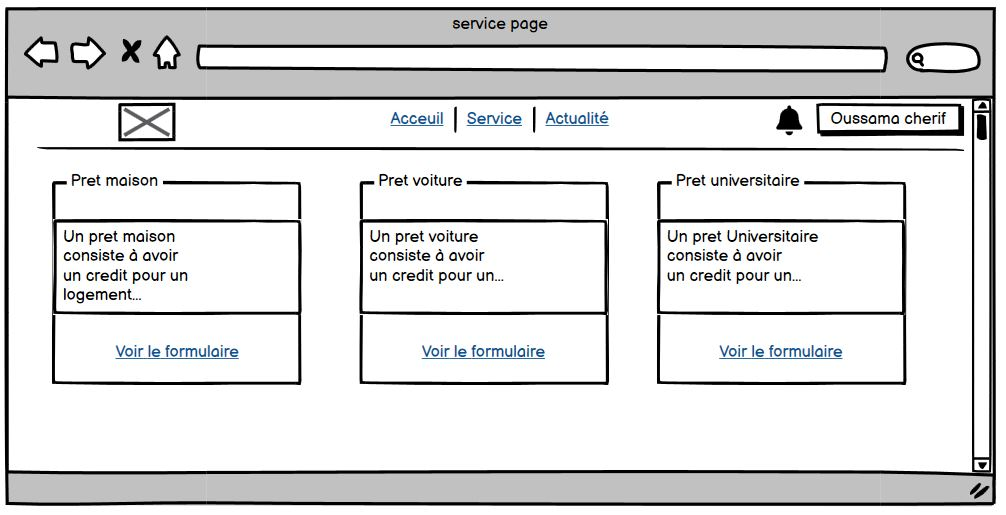
\includegraphics[width=1\textwidth]{figures/service page.JPG} 
    \caption{Prototype of Service Page.}
\end{figure}\

\begin{figure}[h]
    \centering
    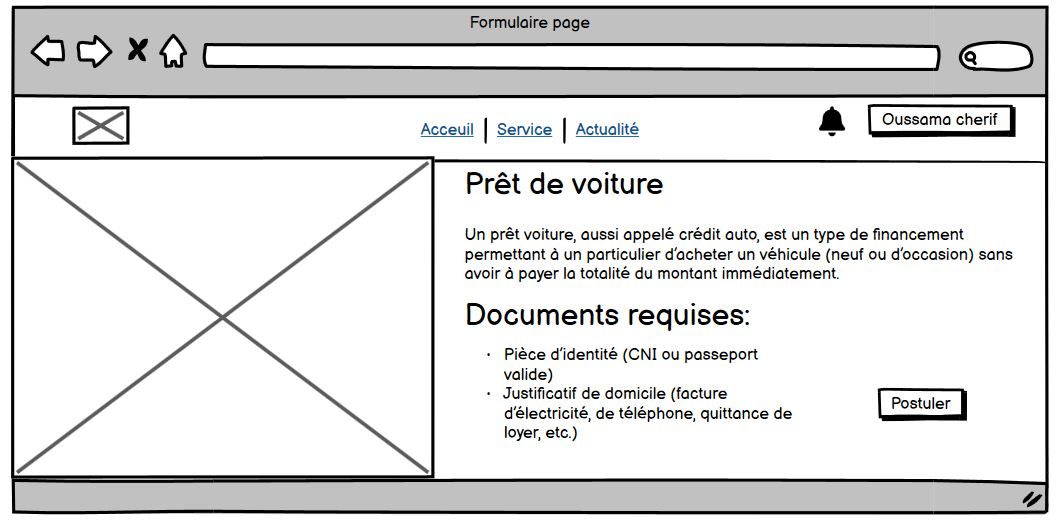
\includegraphics[width=1\textwidth]{figures/formulaire page.JPG}
    \caption{Prototype of form Page.}
\end{figure}\

\begin{figure}[h]
    \centering
    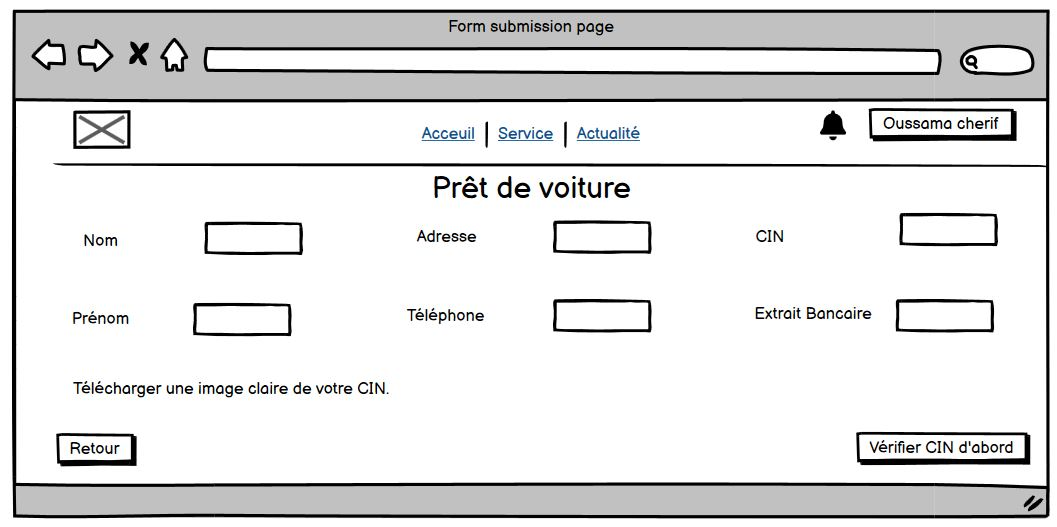
\includegraphics[width=1\textwidth]{figures/form sub page.JPG} 
    \caption{Prototype of form submission Page.}
\end{figure}\
\end{itemize}
\FloatBarrier
\begin{itemize}
    \item Managing the profile prototype
    \begin{figure}[h]
    \centering
    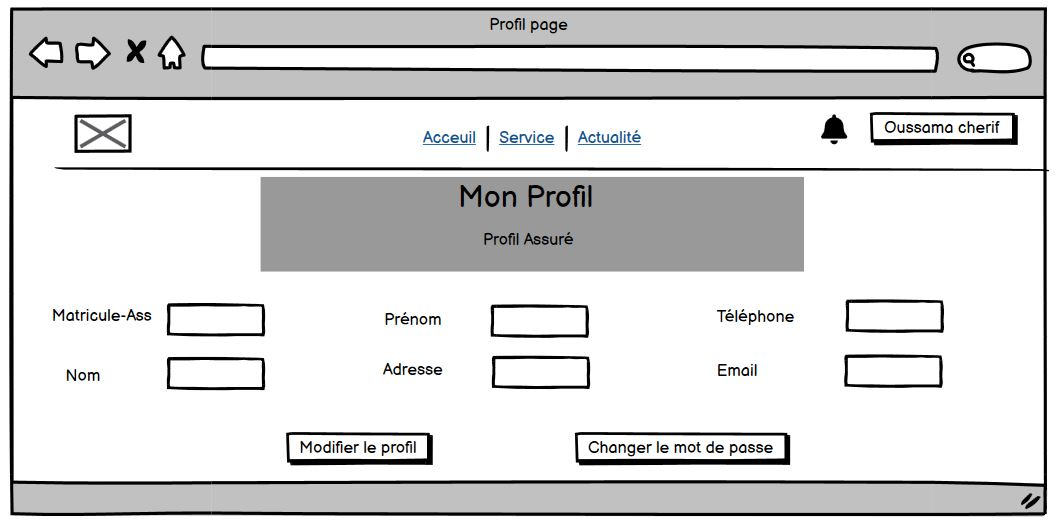
\includegraphics[width=1\textwidth]{figures/profil page.JPG} 
    \caption{Prototype of Profile Page.}
\end{figure}\
\end{itemize}
\clearpage
\begin{itemize}
    \item Review submission prototype 
    \begin{figure}[h]
    \centering
    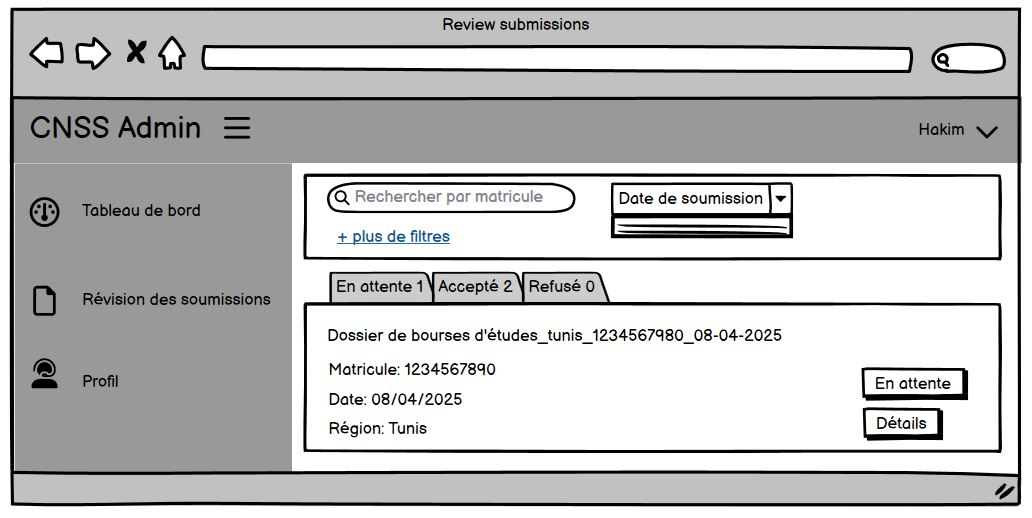
\includegraphics[width=1\textwidth]{figures/review sub.JPG}
    \caption{Prototype of Submission Review Page.}
\end{figure}\
\end{itemize}
\begin{itemize}
    \item Managing internal skateholders prototype\begin{figure}[h!]
    \centering
    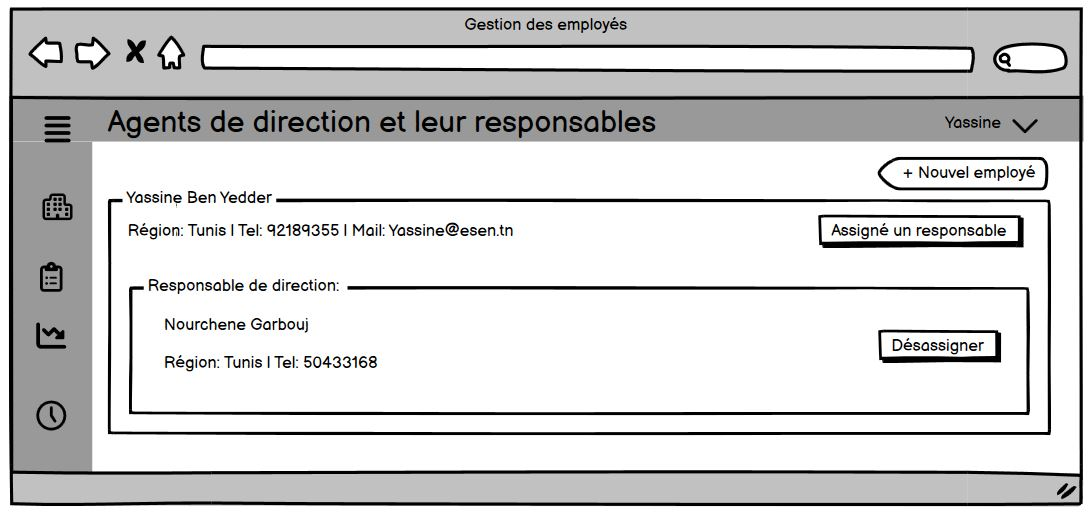
\includegraphics[width=1\textwidth]{figures/ges emp.JPG}
    \caption{Prototype of managing skateholders.}
\end{figure}\
\end{itemize}
\clearpage
\begin{itemize}
    \item managing the submission coordinators\begin{figure}[h!]
    \centering
    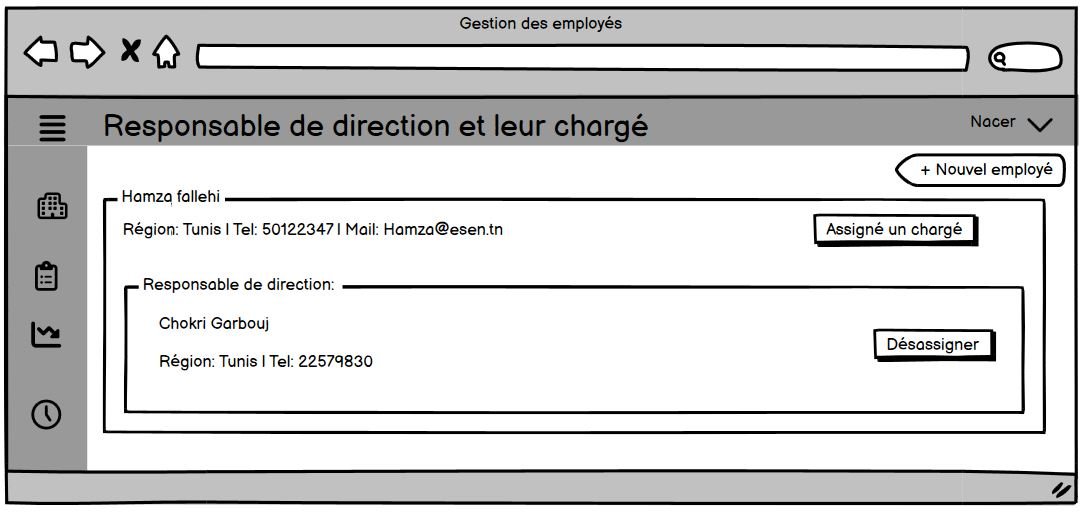
\includegraphics[width=1\textwidth]{figures/ges emp2.JPG}
    \caption{Prototype of managing the submission coordinators.}
\end{figure}\
\end{itemize}

\begin{itemize}
    \item Managing dynamic forms\begin
    {figure}[h]
    \centering
    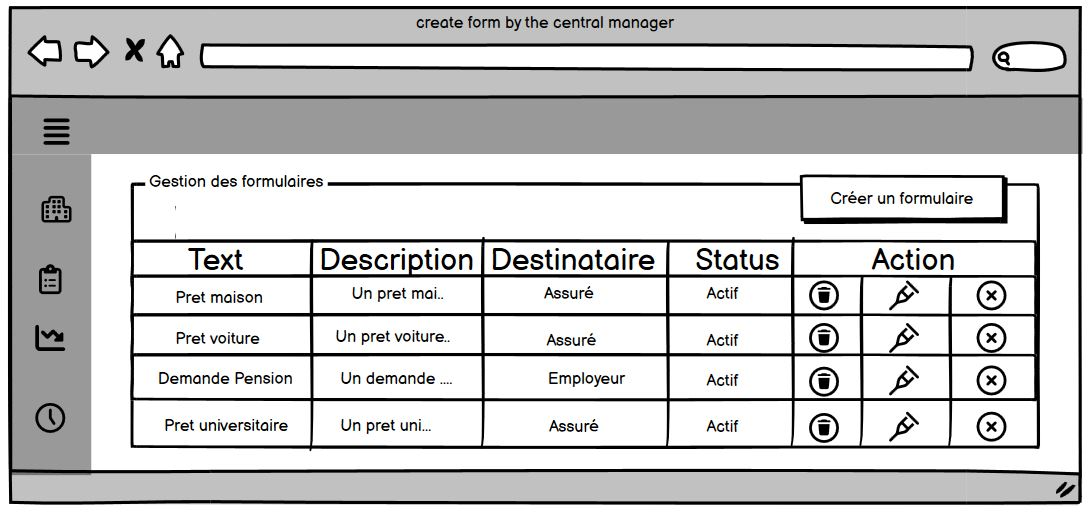
\includegraphics[width=1\textwidth]{figures/create form by the central manager.JPG}
    \caption{Prototype of the creation of a form Page.}
\end{figure}\
\end{itemize}


\clearpage

\section{Use Case Analysis}
For each use case, we will provide a textual description to explain the scenario of each and the exceptions that may occur.
\subsection{Use Case Analysis: "Authenticate"}
\subsubsection{Textual Description of the "Authenticate" Use Case}

\begin{table}[h!]
\centering
\renewcommand{\arraystretch}{1.5}
\begin{tabular}{|c|p{9cm}|}
\hline
\textbf{Use Case} & \textbf{Authenticate} \\ \hline
\textbf{Actor} & Every user of the system. \\ \hline
\textbf{Pre-condition} & The user has login credentials. \\ \hline
\textbf{Post-condition} & The user is authenticated. \\ \hline
\textbf{Main Scenario Description} & 
\begin{tabular}[c]{@{}l@{}} 
1. The system displays the login form. \\
2. The user enters their credentials (email or \\username and password) into the appropriate fields. \\
3. The user submits the form by clicking "Login." \\
4. The system verifies the information entered by the\\ user. \\
5. The system displays the appropriate interface.
\end{tabular} \\ \hline
\textbf{Alternative Scenarios} & 
\begin{tabular}[c]{@{}l@{}} 
4.a. The user enters incomplete data. \\
4.a.1: The system displays an error message. \\
4.a.2: The user repeats step 1 of the main scenario. \\
4.b. The user enters invalid data. \\
4.b.1: The system displays an error message. \\
4.b.2: The user repeats step 1 of the main scenario.
\end{tabular} \\ \hline
\end{tabular}
\caption{Use Case: Authenticate}
\end{table}
\clearpage

\begin{figure}[h!]
    \centering
    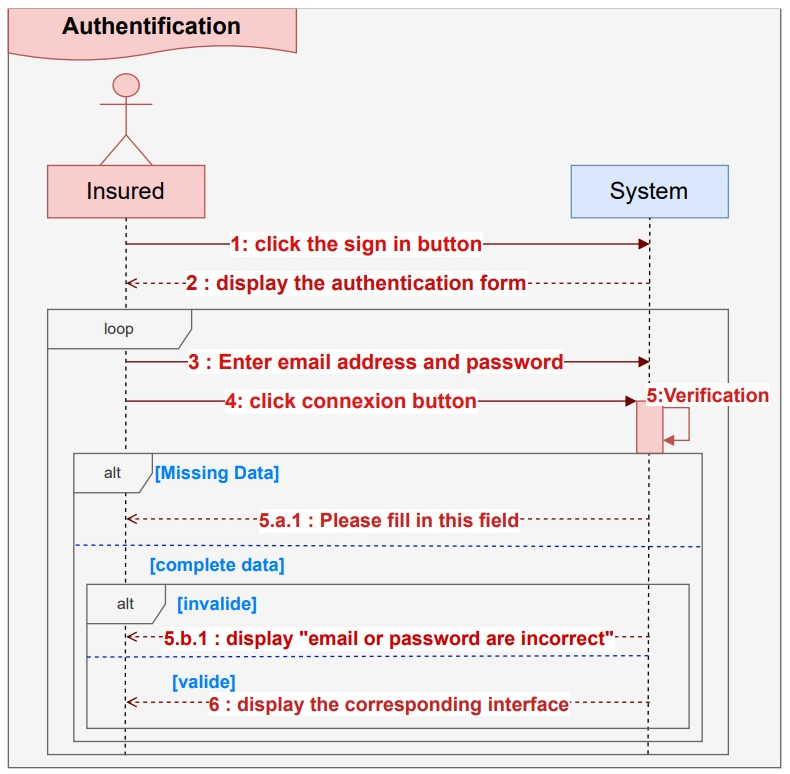
\includegraphics[width=1\textwidth]{figures/seqAuthentification.png}
    \caption{System Sequence Diagram of the "Authenticate" Use Case.}
\end{figure}
\clearpage
\subsection{Use Case Analysis: "Submit a service request"}
\subsubsection{Textual Description of the "Submit a service request" Use Case}

\begin{table}[h!]
\centering
\renewcommand{\arraystretch}{1.5}
\begin{tabular}{|c|p{9cm}|}
\hline
\textbf{Use Case} & \textbf{Submit a service request} \\ \hline
\textbf{Actor} & Insured \\ \hline
\textbf{Pre-condition} & The user is authenticated. \\ \hline
\textbf{Post-condition} & The service request is submitted and sent to the file manager.\\ 
\hline
\textbf{Main Scenario Description} & 
\begin{tabular}[c]{@{}l@{}} 
1. The insured clicks on a specific form \\
2. The system displays the form \\
3. The insured fills in the form \\
4. The insured validates the form by clicking\\ the submit button \\
5. The system verifies the entered information \\
6. The system displays a message indicating that \\the form was submitted successfully \\
\end{tabular} \\ \hline
\textbf{Alternative Scenarios} & 
\begin{tabular}[c]{@{}l@{}} 
4.a. The insured cancels the submission \\
4.a.1: The system cancels the submission. \\
4.a.2: The user repeats step 1 of the main scenario. \\
5.a One of the required fields is empty\\
5.a.1 The system displays an error message.\\
5.a.2 The process returns to step 3 of the main \\scenario.\\
5.b One of the required fields is invalid\\
5.b.1 The system displays an error message.\\
5.b.2 The process returns to step 3 of the main\\ scenario.\\
\end{tabular} \\ \hline
\end{tabular}
\caption{Use Case: Submit a service request}
\end{table}
\clearpage

\begin{figure}[h!]
    \centering
    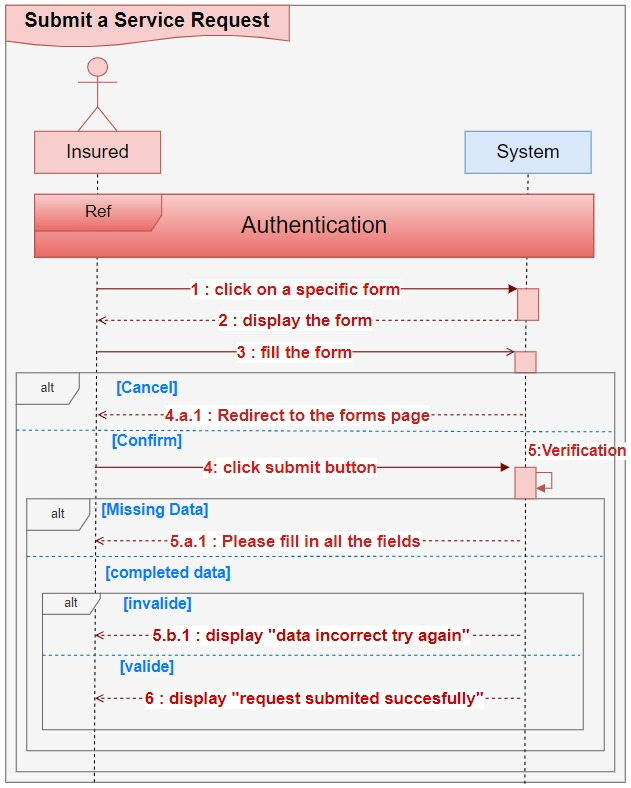
\includegraphics[width=1\textwidth]{figures/seqSubmits_service_request.png}
    \caption{System Sequence Diagram of the "Submit a service request" Use Case.}
\end{figure}\
\clearpage


\subsection{Use Case Analysis: "Manage Profile"}
\subsubsection{Refinement of the use case 'Manage Profile'}
\begin{figure}[h!]
    \centering
    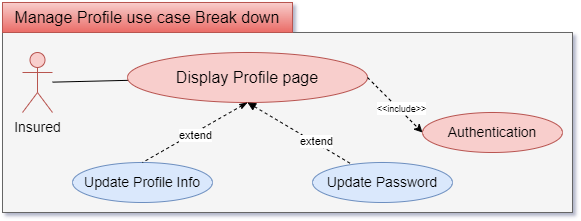
\includegraphics[width=1\textwidth]{figures/bd_manage_profile.png}
    \caption{Refinement of the use case 'Manage Profile'}
\end{figure}\


\subsubsection{Textual Description of the "Display profile page" Use Case}

\begin{table}[h!]
\centering
\renewcommand{\arraystretch}{1.5}
\begin{tabular}{|c|p{9cm}|}
\hline
\textbf{Use Case} & \textbf{Display profile page} \\ \hline
\textbf{Actor} & Every user of the system. \\ \hline
\textbf{Pre-condition} & The user is authenticated. \\ \hline
\textbf{Post-condition} & the profile page is displayed.\\ 
\hline
\textbf{Main Scenario Description} & 
\begin{tabular}[c]{@{}l@{}} 
1. The user clicks on the "My Profile" element \\
2. The system displays the profile page \\
\end{tabular} \\ \hline
\textbf{Alternative Scenarios} & 
\begin{tabular}[c]{@{}l@{}} 
None \\
\end{tabular} \\ \hline
\end{tabular}
\caption{Use Case: Display Profile page}
\end{table}
\clearpage

\begin{figure}[h!]
    \centering
    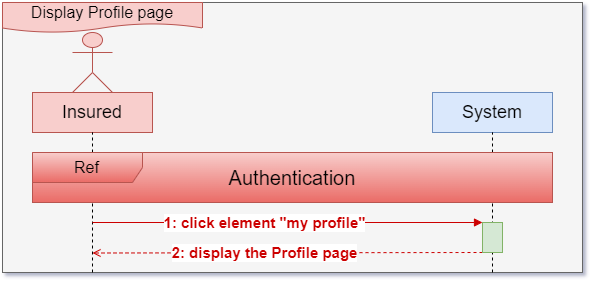
\includegraphics[width=1\textwidth]{figures/seqDisplay_profile.png}
    \caption{System Sequence Diagram of the "Display Profile page" Use Case.}
\end{figure}
\clearpage


\subsubsection{Textual Description of the "Update Profile" Use Case}

\begin{table}[h!]
\centering
\renewcommand{\arraystretch}{1.5}
\begin{tabular}{|c|p{8cm}|}
\hline
\textbf{Use Case} & \textbf{Update Profile} \\ \hline
\textbf{Actor} & Insured \\ \hline
\textbf{Pre-condition} & The insured is logged in and on their profile page. \\ \hline
\textbf{Post-condition} & The profile information is successfully updated. \\ \hline
\textbf{Main Scenario Description} & 
\begin{tabular}[c]{@{}l@{}} 
1. The insured clicks the "Update my profile" \\button. \\
2. The system displays a form to update profile\\ information. \\
3. The insured updates their profile information. \\
4. The insured clicks the "Confirm" button. \\
5. The system verifies the provided data. \\
6. The system displays a success message: \\"Profile updated\\ successfully." \\
\end{tabular} \\ \hline
\textbf{Alternative Scenarios} & 
\begin{tabular}[c]{@{}l@{}} 
4.a. The insured clicks "Cancel" instead of \\confirming. \\
4.a.1. The system redirects the insured back to \\the profile page. \\[0.2cm]
5.a. Some required fields are missing. \\
5.a.1. The system displays an error message:\\ "Please fill in this field." \\
5.a.2. The process returns to step 3 of the main \\scenario. \\
\end{tabular} \\ \hline
\end{tabular}
\caption{Use Case: Update Profile}
\end{table}
\clearpage

\begin{figure}[h!]
    \centering
    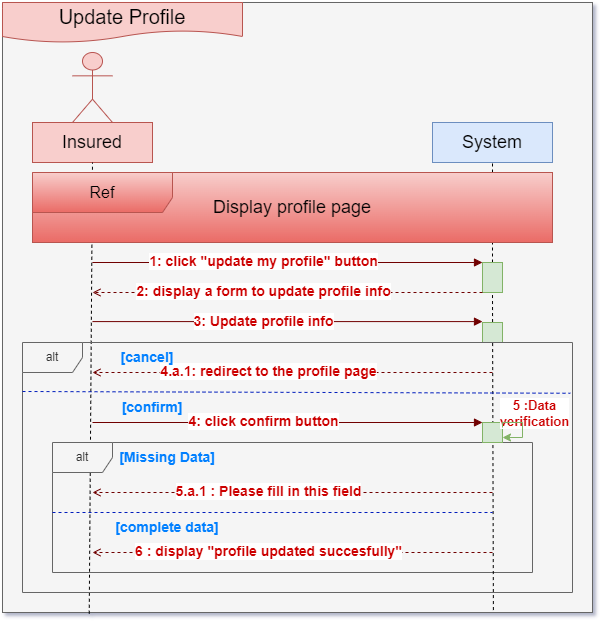
\includegraphics[width=1\textwidth]{figures/seqUpdate_profile.png}
    \caption{System Sequence Diagram of the "Update Profile" Use Case.}
\end{figure}
\clearpage


\subsubsection{Textual Description of the "Update Password" Use Case}
\begin{table}[h!]
\centering
\renewcommand{\arraystretch}{1.5}
\begin{tabular}{|c|p{9cm}|}
\hline
\textbf{Use Case} & \textbf{Update Password} \\ \hline
\textbf{Actor} & Insured \\ \hline
\textbf{Pre-condition} & The insured is logged in and on their profile page. \\ \hline
\textbf{Post-condition} & The password is successfully updated. \\ \hline
\textbf{Main Scenario Description} & 
\begin{tabular}[c]{@{}l@{}} 
1. The insured clicks the "Update my password" \\button. \\
2. The system displays a form to update the password. \\
3. The insured fills in the form. \\
4. The insured clicks the "Confirm" button. \\
5. The system verifies the provided data. \\
6. The system displays a success message: "Password \\updated successfully." \\
\end{tabular} \\ \hline
\textbf{Alternative Scenarios} & 
\begin{tabular}[c]{@{}l@{}} 
4.a. The insured clicks "Cancel". \\
4.a.1. The system redirects the user back to the profile\\ page. \\[0.2cm]
5.a. Some required fields are missing. \\
5.a.1. The system displays an error message: "Please \\fill in this field." \\
5.a.2. The process returns to step 3 of the main \\scenario. \\[0.2cm]
5.b. Provided data is invalid. \\ 
5.b.1. If the passwords do not match: \\
The system displays an error message: "Password \\doesn't match." \\
5.b.2. If the password is less than 8 characters: \\
The system displays: "Password must be 8 characters \\at least." \\
5.b.3. The process returns to step 3 of the main \\scenario. \\
\end{tabular} \\ \hline
\end{tabular}
\caption{Use Case: Update Password}
\end{table}
\clearpage

\begin{figure}[h!]
    \centering
    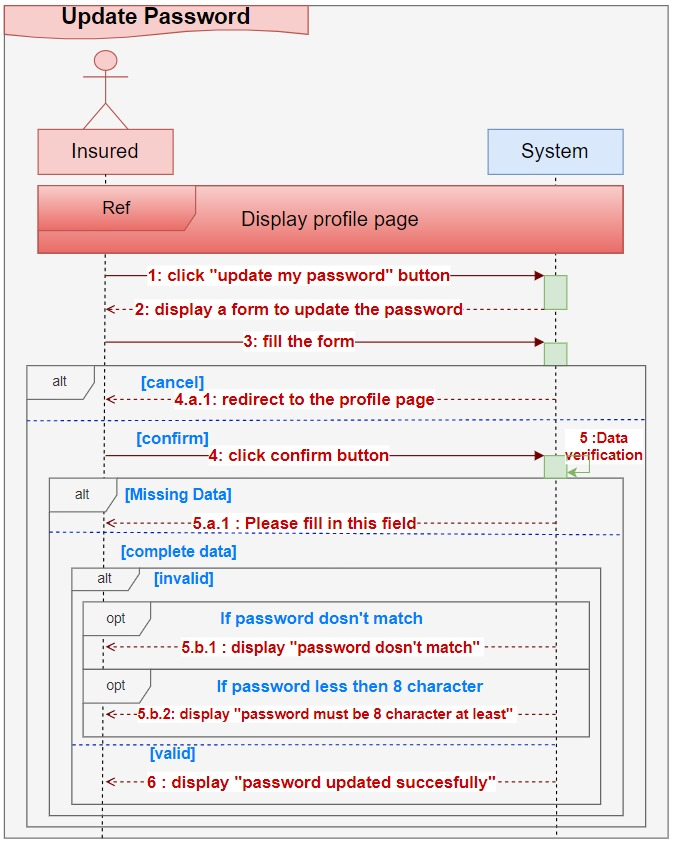
\includegraphics[width=1\textwidth]{figures/sequpdate_password.png}
    \caption{System Sequence Diagram of the "Update Password" Use Case.}
\end{figure}
\clearpage

\subsection{Use Case Analysis: "Review a Submission"}
\subsubsection{Refinement of the use case 'Review a submission'}
\begin{figure}[h!]
    \centering
    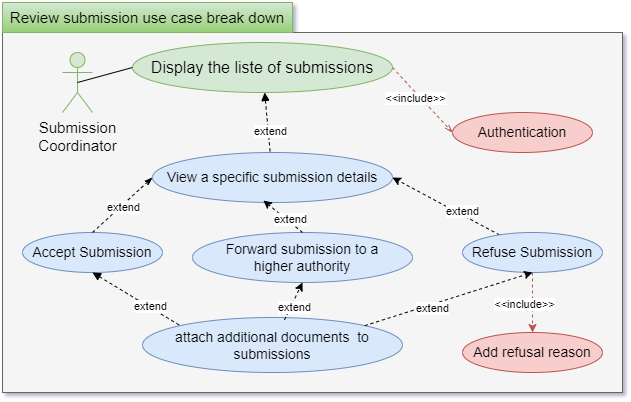
\includegraphics[width=1\textwidth]{figures/bdreview_submission.drawio.png}
    \caption{Refinement of the use case 'Review a submission'}
\end{figure}\


\subsubsection{Textual Description of the "Display submission details" Use Case}

\begin{table}[h!]
\centering
\renewcommand{\arraystretch}{1.5}
\begin{tabular}{|c|p{9cm}|}
\hline
\textbf{Use Case} & \textbf{Display submission details} \\ \hline
\textbf{Actor} & Submission Coordinators \\ \hline
\textbf{Pre-condition} & The user is authenticated. \\ \hline
\textbf{Post-condition} & the submission details is displayed.\\ 
\hline
\textbf{Main Scenario Description} & 
\begin{tabular}[c]{@{}l@{}} 
1. The user clicks on "Details" button of a specific \\submission \\
2. The system displays the submission details \\
\end{tabular} \\ \hline
\textbf{Alternative Scenarios} & 
\begin{tabular}[c]{@{}l@{}} 
None \\
\end{tabular} \\ \hline
\end{tabular}
\caption{Use Case: Display submission details}
\end{table}
\clearpage

\begin{figure}[h!]
    \centering
    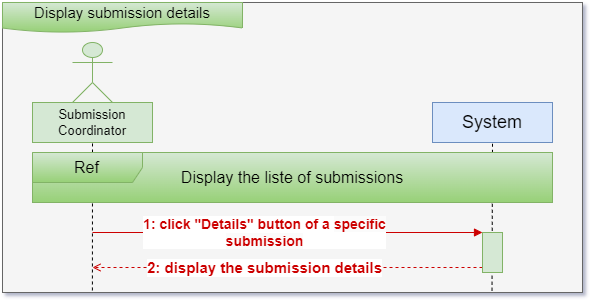
\includegraphics[width=1\textwidth]{figures/seqdisplay_submission_details.png}
    \caption{system Sequence Diagram of the "Display submission details" Use Case.'}
\end{figure}
\clearpage


\subsubsection{Textual Description of the "Refuse submission" Use Case}

\begin{table}[h!]
\centering
\renewcommand{\arraystretch}{1.5}
\begin{tabular}{|c|p{8cm}|}
\hline
\textbf{Use Case} & Refuse Submission \\ \hline
\textbf{Actor} & Submission Coordinator \\ \hline
\textbf{Pre-condition} & The coordinator is logged in and viewing the submission details. \\ \hline
\textbf{Post-condition} & The submission is marked as refused, and a reason (and optionally, documents) is saved. \\ \hline
\textbf{Main Scenario Description} & 
\begin{tabular}[c]{@{}l@{}} 
1. The coordinator clicks the "Refuse" button. \\
2. The system displays a textbox for the refusal \\reason. \\
3. The coordinator enters the refusal reason. \\
4. The coordinator clicks the "Confirm" button. \\
5. The system displays the message: \\"Submission reviewed successfully." \\
\end{tabular} \\ \hline
\textbf{Alternative Scenarios} & 
\begin{tabular}[c]{@{}l@{}} 
3.a. The coordinator wants to attach additional \\documents. \\
3.a.1. The coordinator attaches the documents. \\[0.2cm]
4.a. The coordinator clicks "Cancel". \\
4.a.1. The system redirects to the submission\\ list. \\
\end{tabular} \\ \hline
\end{tabular}
\caption{Use Case: Refuse Submission}
\end{table}

\clearpage
\begin{figure}[h!]
    \centering
    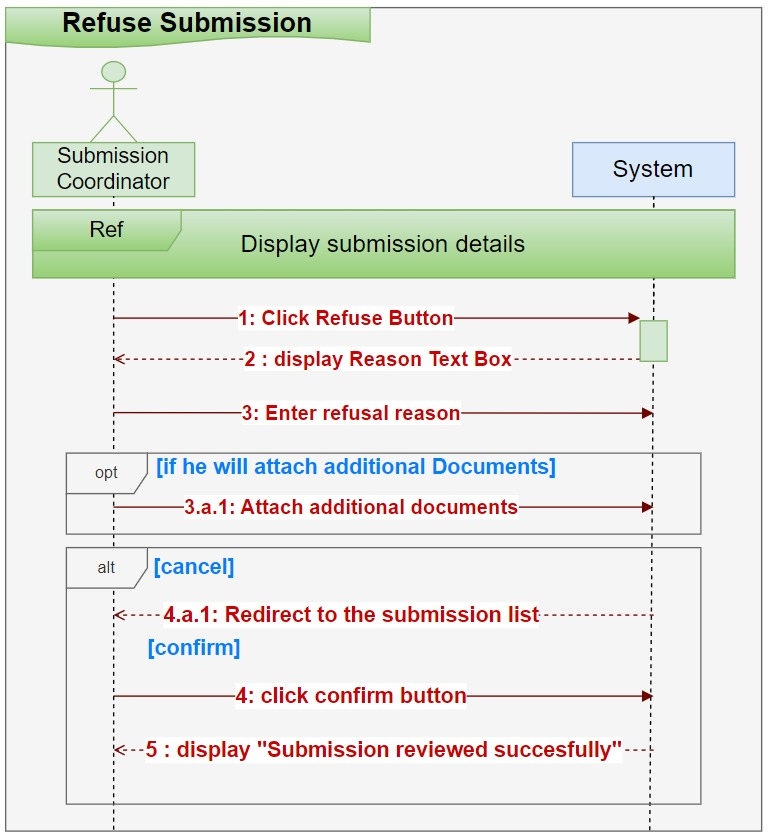
\includegraphics[width=1\textwidth]{figures/seqrefuse_submission.png}
    \caption{system Sequence Diagram of the "Refuse Submission" Use Case.'}
\end{figure}
\clearpage


\subsubsection{Textual Description of the "Escalate submission to a higher authority" Use Case}

\begin{table}[h!]
\centering
\renewcommand{\arraystretch}{1.5}
\begin{tabular}{|c|p{8cm}|}
\hline
\textbf{Use Case} & Escalate Submission to a Higher Authority \\ \hline
\textbf{Actor} & Submission Coordinator \\ \hline
\textbf{Pre-condition} & The coordinator is logged in and viewing the submission details. \\ \hline
\textbf{Post-condition} & The submission is Escalated to a higher authority successfully. \\ \hline
\textbf{Main Scenario Description} & 
\begin{tabular}[c]{@{}l@{}} 
1. The coordinator clicks the "Escalate" button. \\
2. The coordinator clicks the "Confirm" button. \\
3. The system displays the message: \\"Submission reviewed successfully." \\
\end{tabular} \\ \hline
\textbf{Alternative Scenarios} & 
\begin{tabular}[c]{@{}l@{}} 
1.a. The coordinator wants to attach additional\\ documents. \\
1.a.1. The coordinator attaches the documents. \\[0.2cm]
2.a. The coordinator clicks "Cancel". \\
2.a.1. The system redirects to the submission \\list. \\
\end{tabular} \\ \hline
\end{tabular}
\caption{Use Case: Escalate Submission to a Higher Authority}
\end{table}

\clearpage
\begin{figure}[h!]
    \centering
    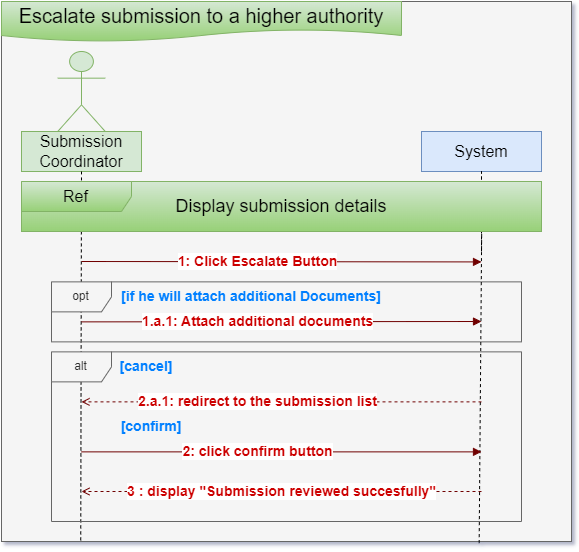
\includegraphics[width=1\textwidth]{figures/seqescalate_submission.png}
    \caption{system Sequence Diagram of the "Escalate Submission to a Higher Authority" \centering Use Case.}
\end{figure}
\clearpage
\subsection{Use Case Analysis: "Manage internal skateholders"}
\subsubsection{Refinement of the use case 'Manage internal skateholders'}
\begin{figure}[h!]
    \centering
    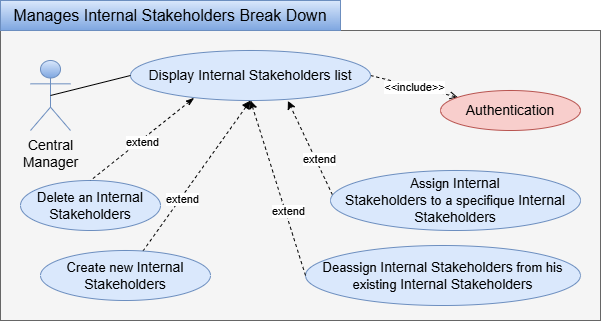
\includegraphics[width=1\textwidth]{figures/bdManages Internal Stakeholders.png}
    \caption{Refinement of the use case 'Manage Profile'}
\end{figure}\
\clearpage

\subsubsection{Textual Description of the "Create new internal stakeholders" Use Case}
\begin{table}[h!]
\centering
\renewcommand{\arraystretch}{1.5}
\begin{tabular}{|c|p{8cm}|}
\hline
\textbf{Use Case} & Create Internal Stakeholders \\ \hline
\textbf{Actor} & Central Manager \\ \hline
\textbf{Pre-condition} & The user is authenticated and on the Internal Stakeholders List page. \\ \hline
\textbf{Post-condition} & A new internal stakeholder is created and a confirmation message is displayed. \\ \hline
\textbf{Main Scenario Description} & 
\begin{tabular}[c]{@{}l@{}}
1. The user clicks on the "Create Internal \\Stakeholders" button. \\
2. The system displays a form to create a new \\internal stakeholder. \\
3. The user fills the form. \\
4. The user clicks the "Confirm" button. \\
5. The system verifies the data. \\
6. The system displays "Internal Stakeholder \\created". \\
\end{tabular} \\ \hline
\textbf{Alternative Scenarios} & 
\begin{tabular}[c]{@{}l@{}}
\textbf{4.a.} The user clicks "Cancel": \\
\quad 4.a.1. Redirect to the internal stakeholders \\list. \\
\textbf{5.a.} Data is incomplete: \\
\quad 5.a.1. System prompts: "Please fill in this \\field". \\
\end{tabular} \\ \hline
\end{tabular}
\caption{Use Case: Create Internal Stakeholders}
\end{table}
\clearpage
\begin{figure}[h!]
    \centering
    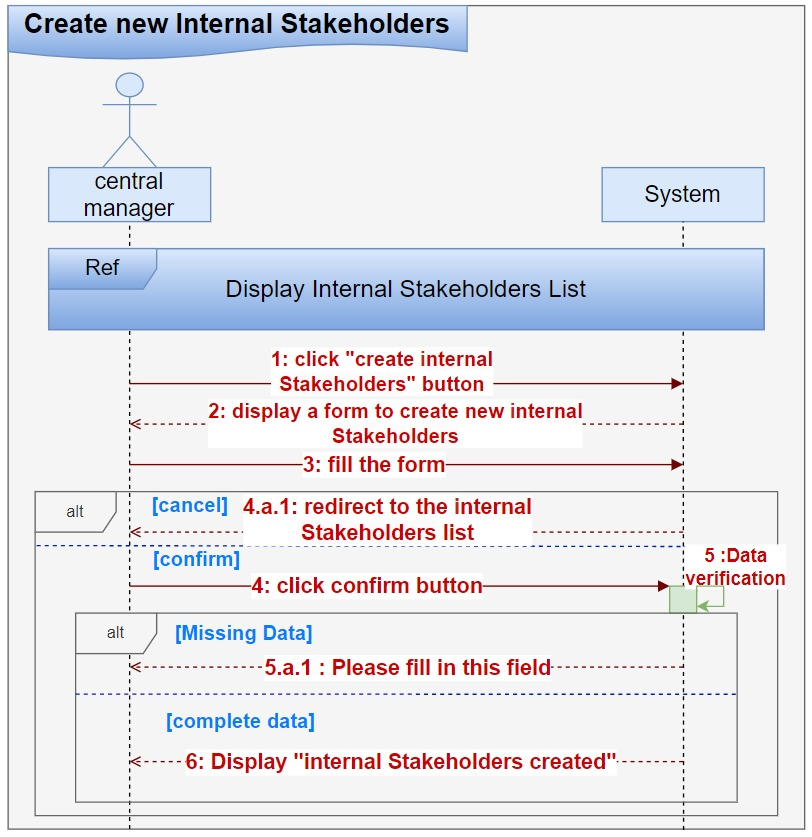
\includegraphics[width=1\textwidth]{figures/seqcreate internal skateholder.png}
    \caption{System Sequence Diagram of the "Create Internal Stakeholders" Use Case.}
\end{figure}
\clearpage


\subsubsection{Textual Description of the "Delete an internal stakeholders" Use Case}
\begin{table}[h!]
\centering
\renewcommand{\arraystretch}{1.5}
\begin{tabular}{|c|p{8cm}|}
\hline
\textbf{Use Case} & Delete an Internal Stakeholder \\ \hline
\textbf{Actor} & Central Manager \\ \hline
\textbf{Pre-condition} & The user is authenticated and viewing the Internal Stakeholders List. \\ \hline
\textbf{Post-condition} & The selected internal stakeholder is deleted, or the operation is canceled. \\ \hline
\textbf{Main Scenario Description} & 
\begin{tabular}[c]{@{}l@{}}
1. The user clicks "Delete" on an internal \\stakeholder. \\
2. The system displays a confirmation message:\\ "Are you sure you want to delete this \\employee?" \\
3. The user selects a choice (Confirm or Cancel). \\
4. If confirmed, the system displays "Employee\\ deleted successfully". \\
\end{tabular} \\ \hline
\textbf{Alternative Scenarios} & 
\begin{tabular}[c]{@{}l@{}}
\textbf{4.a.} The user clicks "Cancel": \\
\quad 4.a.1. The system redirects to the Internal \\Stakeholders List. \\
\end{tabular} \\ \hline
\end{tabular}
\caption{Use Case: Delete an Internal Stakeholder}
\end{table}
\clearpage
\begin{figure}[h!]
    \centering
    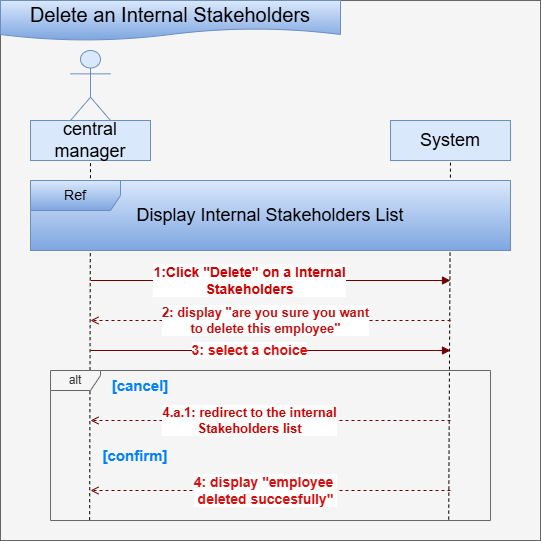
\includegraphics[width=1\textwidth]{figures/seqdelete internal.png}
    \caption{System Sequence Diagram of the "Delete an Internal Stakeholder" Use Case.}
\end{figure}
\clearpage

\subsubsection{Textual Description of the "Assign an internal stakeholder to another" Use Case}
\begin{table}[h!]
\centering
\renewcommand{\arraystretch}{1.5}
\begin{tabular}{|c|p{8cm}|}
\hline
\textbf{Use Case} & Assign an Internal Stakeholder to another \\ \hline
\textbf{Actor} & Central Manager \\ \hline
\textbf{Pre-condition} & The Central Manager is authenticated and viewing the Internal Stakeholders List. \\ \hline
\textbf{Post-condition} & The stakeholder is either successfully assigned or a validation error is shown. \\ \hline
\textbf{Main Scenario Description} & 
\begin{tabular}[c]{@{}l@{}}
1. The Central Manager selects the assignment \\type and submits. \\
2. The system performs data verification. \\
3. If the data is valid, the system displays a \\success message. \\
\end{tabular} \\ \hline
\textbf{Alternative Scenarios} & 
\begin{tabular}[c]{@{}l@{}}
\textbf{3.a.} If the assignment is invalid due to region \\conflict:
\quad 3.a.1. Display: "File manager should\\ have the same region as office supervisor." \\
\end{tabular} \\ \hline
\end{tabular}
\caption{Use Case: Assign an Internal Stakeholder to another}
\end{table}

\clearpage
\begin{figure}[h!]
    \centering
    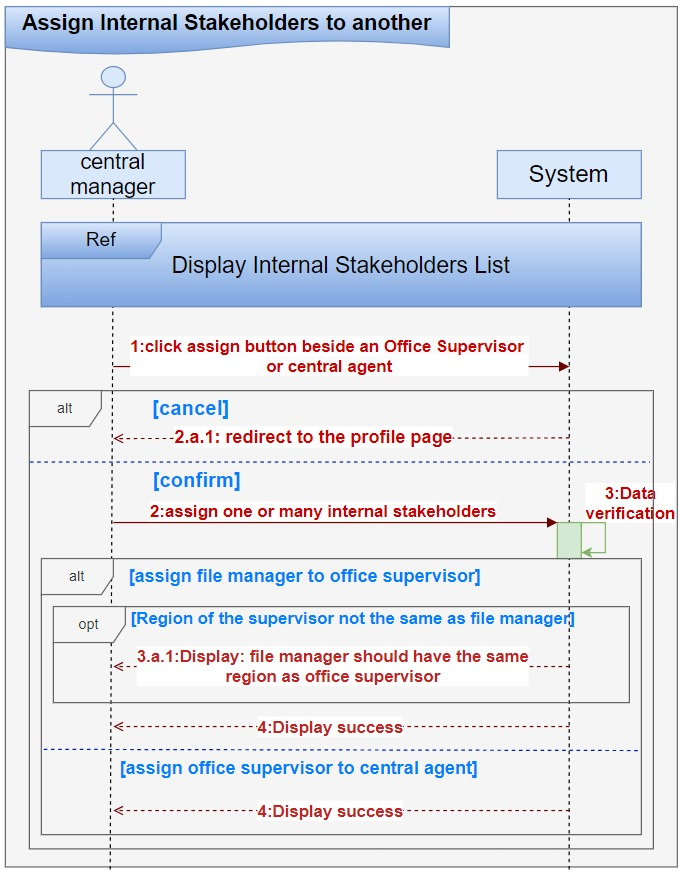
\includegraphics[width=1\textwidth]{figures/seqassign internal stakeholders.png}
    \caption{System Sequence Diagram of the "Assign an internal stakeholder to another" Use Case.}
\end{figure}
\clearpage

\subsection{Use Case Analysis: "Manage Dynamic Forms"}
\subsubsection{Refinement of the use case 'Manage dynamic forms'}
\begin{figure}[h!]
    \centering
    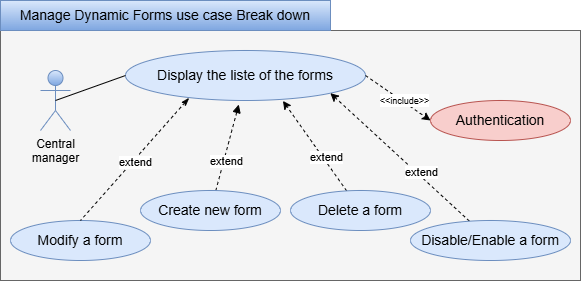
\includegraphics[width=1\textwidth]{figures/bdmanages dynamic forms-Break down.png}
    \caption{Refinement of the use case 'Manage Dynamic forms'}
\end{figure}\

\clearpage
\subsubsection{Textual Description of the "Create a new form" Use Case}
\begin{table}[h!]
\centering
\renewcommand{\arraystretch}{1.5}
\begin{tabular}{|c|p{8cm}|}
\hline
\textbf{Use Case} & Create a New Form \\ \hline
\textbf{Actor} & Central Manager \\ \hline
\textbf{Pre-condition} & The Central Manager is authenticated and on the "Forms List" page. \\ \hline
\textbf{Post-condition} & A new form is created and displayed in the list, or the operation is canceled. \\ \hline
\textbf{Main Scenario Description} & 
\begin{tabular}[c]{@{}l@{}}
1. The Central Manager clicks "Add new form". \\
2. The system displays a form to add a new \\form. \\
3. The Central Manager fills in the form. \\
4. The Central Manager clicks the "Submit" \\button. \\
5. The system verifies the submitted data. \\
6. If the data is complete, the system displays \\"Form created successfully". \\
\end{tabular} \\ \hline
\textbf{Alternative Scenarios} & 
\begin{tabular}[c]{@{}l@{}}
\textbf{4.a.} If the Central Manager clicks "Cancel": \\
\quad 4.a.1. The system redirects to the forms list. \\
\textbf{5.a.} If required data is missing: \\
\quad 5.a.1. The system displays a message:\\ "Please fill in \\this field". \\
\end{tabular} \\ \hline
\end{tabular}
\caption{Use Case: Create a New Form}
\end{table}

\clearpage
\begin{figure}[h!]
    \centering
    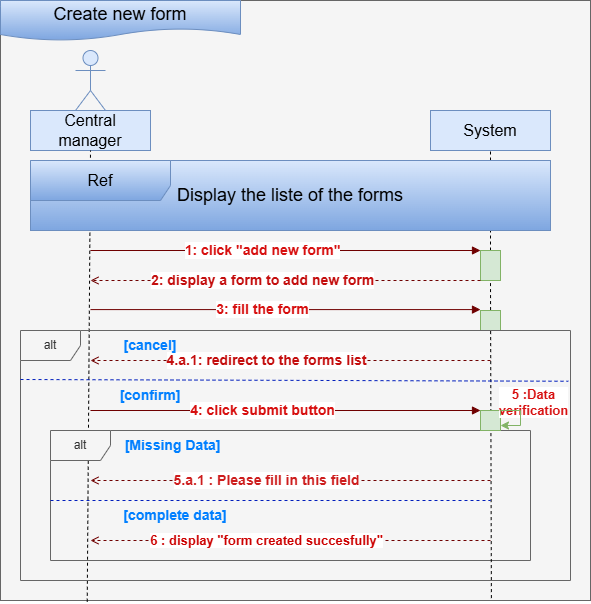
\includegraphics[width=1\textwidth]{figures/seqcreate a form..png}
    \caption{System Sequence Diagram of the "Create a new form " Use Case.}
\end{figure}
\clearpage


\subsubsection{Textual Description of the "Disable/Enable a form" Use Case}
\begin{table}[h!]
\centering
\renewcommand{\arraystretch}{1.5}
\begin{tabular}{|c|p{10cm}|}
\hline
\textbf{Use Case} & Disable/Enable a Form \\ \hline
\textbf{Actor} & Central Manager \\ \hline
\textbf{Pre-condition} & The Central Manager is authenticated and on the "Forms List" page. \\ \hline
\textbf{Post-condition} & The selected form is either disabled or enabled successfully, and the user receives a confirmation message. \\ \hline
\textbf{Main Scenario Description} & 
\begin{tabular}[c]{@{}l@{}}
1. The Central Manager clicks the "disable" button. \\
2. The system displays the message: "Form disabled \\successfully". \\
\end{tabular} \\ \hline
\textbf{Alternative Scenarios} & 
\begin{tabular}[c]{@{}l@{}}
\textbf{2.a.} If the system encounters an error: \\
\quad 2.a.1. The system displays an error message indicating\\ failure to disable the form. \\
\end{tabular} \\ \hline
\end{tabular}
\caption{Use Case: Disable/Enable a Form}
\end{table}
\begin{figure}[h!]
    \centering
    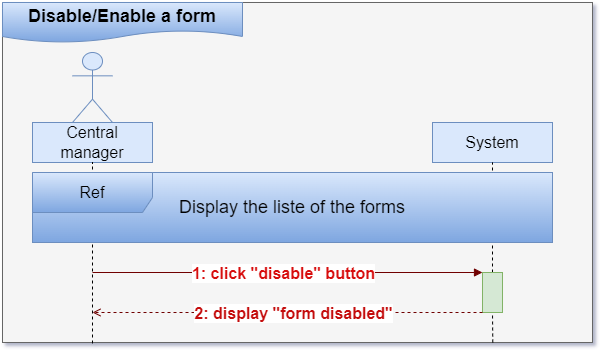
\includegraphics[width=1\textwidth]{figures/seqDisableenable a form.png}
    \caption{System Sequence Diagram of the "Disable/Enable a form " Use Case.}
\end{figure}
\clearpage

\section{Design of Use Cases}
 We proceed to the next step, where we will create the class diagrams involved for each actor, the detailed sequence diagrams of the use cases, and an object class diagram for the first sprint, following the creation of the system sequence diagrams and the textual descriptions of the use cases in the previous section.
 \subsection{The participant Class Diagram}
 \textbf{\textit{"The involvement class diagram is especially significant because it serves as a link between the use cases and software design diagrams, including interaction diagrams and the design class diagram.  Boundary, control, and entity classes are the three categories of analysis classes that are represented in the involved class diagram, along with their relationships."}}\cite{samplewebs6}
 \subsubsection{Participant class Diagram for the use case "Authenticate"}
 \begin{figure}[h!]
    \centering
    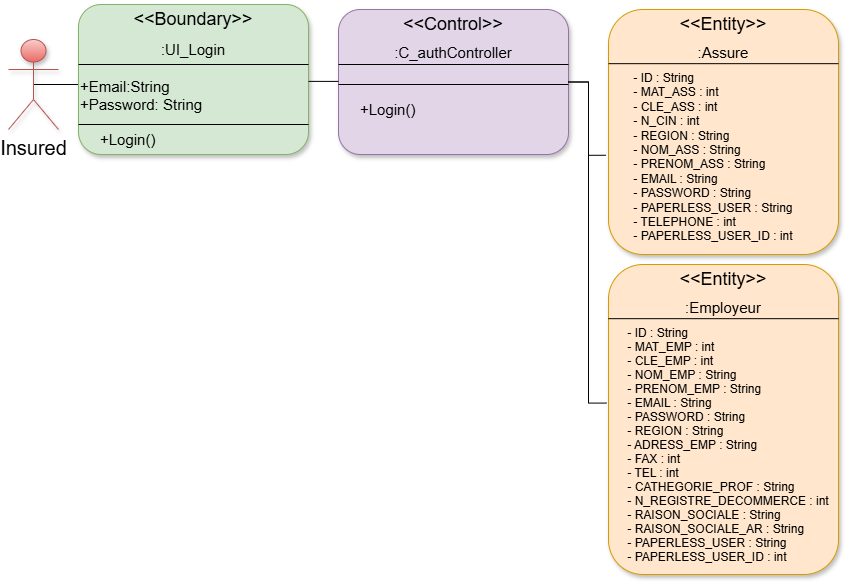
\includegraphics[width=1\textwidth]{figures/dc auth.png}
    \caption{Participant class Diagram for the use case "Authenticate"}
\end{figure}

\subsubsection{Participant class Diagram for the use case "Submit a service request"}
 \begin{figure}[h!]
    \centering
    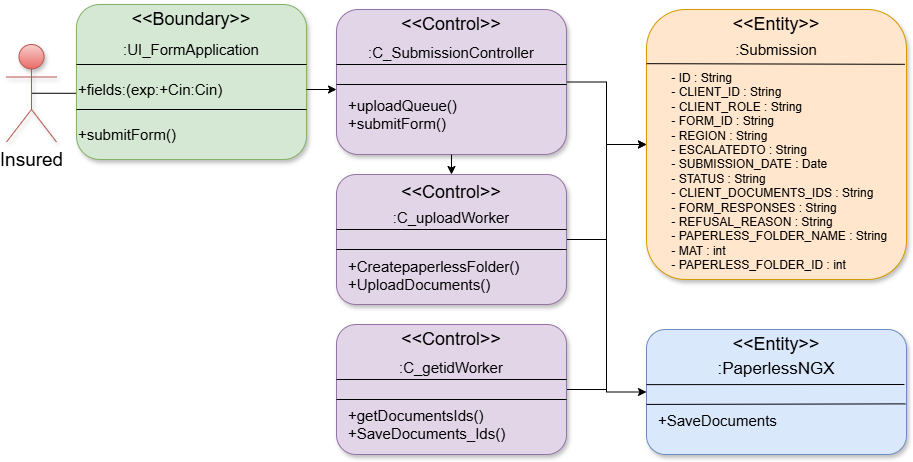
\includegraphics[width=1\textwidth]{figures/dc Submits a service request.png}
    \caption{Participant class Diagram for the use case "Submit a service request"}
\end{figure}

\subsubsection{Participant class Diagram for the use case "Manage Profile"}
 \begin{figure}[h!]
    \centering
    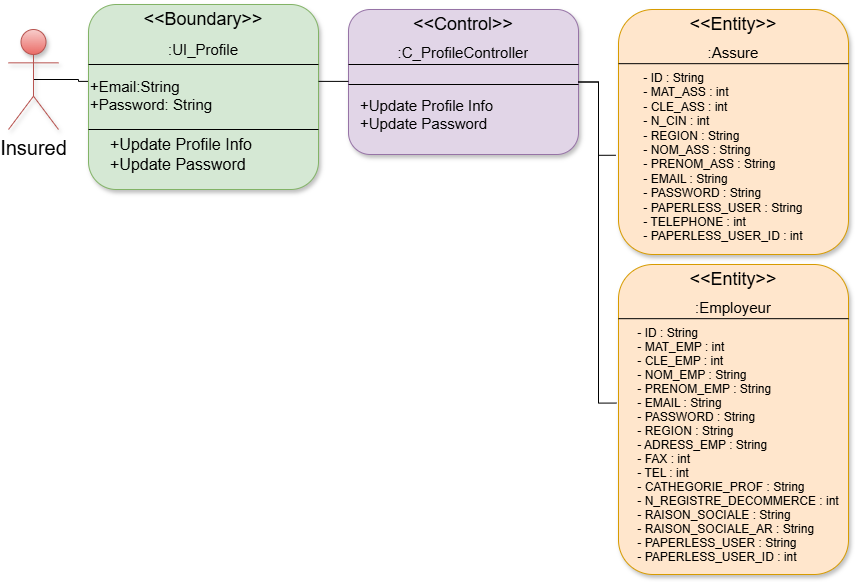
\includegraphics[width=1\textwidth]{figures/dc manage profile.png}
    \caption{Participant class Diagram for the use case "Manage Profile"}
\end{figure}
\clearpage
\subsubsection{Participant class Diagram for the use case "Review Submission"}
 \begin{figure}[h!]
    \centering
    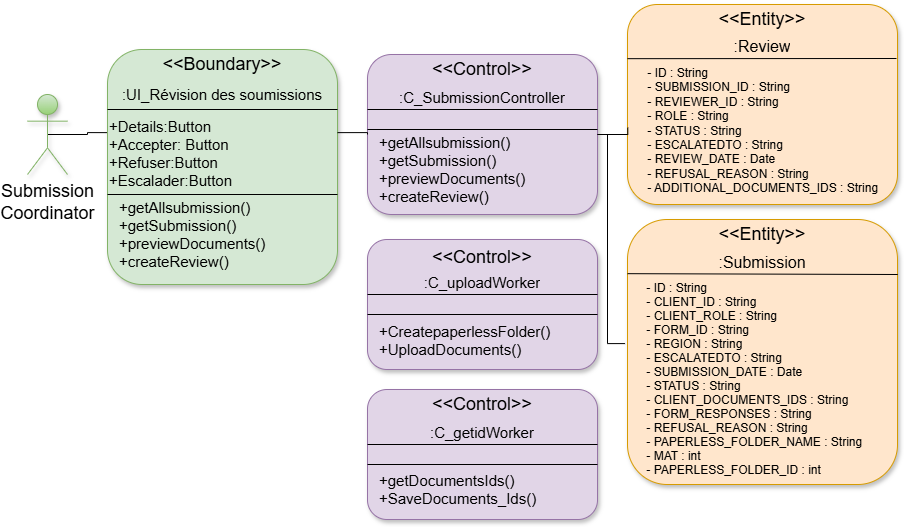
\includegraphics[width=1\textwidth]{figures/dc review submission.png}
    \caption{Participant class Diagram for the use case "Review Submission"}
\end{figure}

\subsubsection{Participant class Diagram for the use case "Manage Dynamic Forms"}
 \begin{figure}[h!]
    \centering
    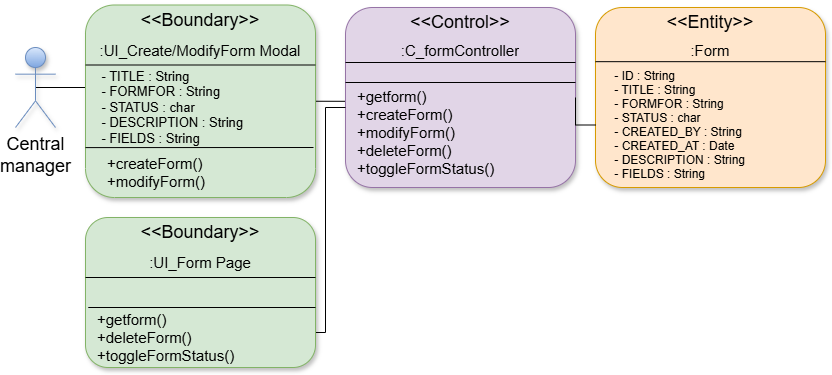
\includegraphics[width=1\textwidth]{figures/dc manageform.png}
    \caption{Participant class Diagram for the use case "Manage Dynamic Forms}
\end{figure}
\clearpage

\subsubsection{Participant class Diagram for the use case "Manage Internal Stakeholders"}
 \begin{figure}[h!]
    \centering
    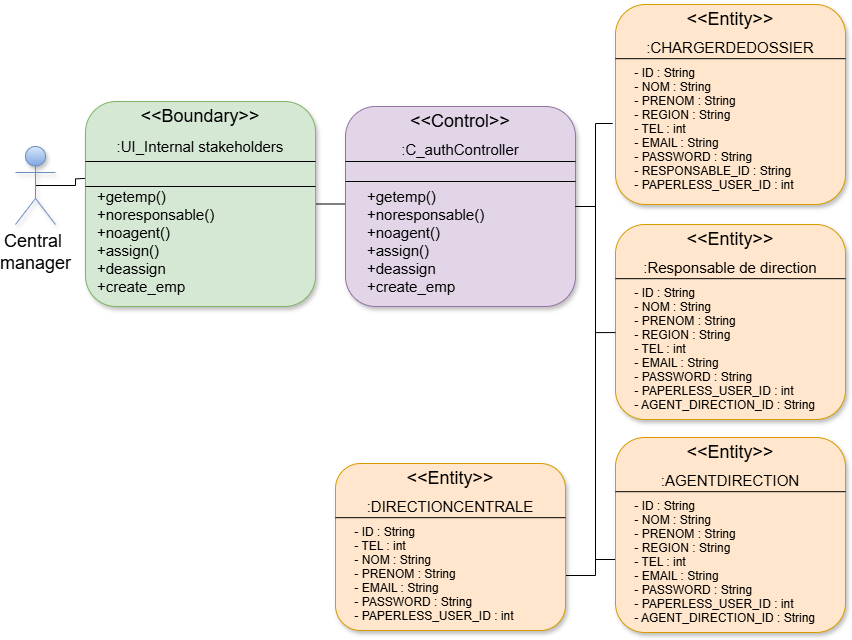
\includegraphics[width=1\textwidth]{figures/dc Manages Internal Stakeholders.png}
    \caption{Participant class Diagram for the use case "Manage Internal Stakeholders}
\end{figure}

\subsection{Detailed Sequence Diagram}
\subsubsection{Detailed sequence diagram of the 'Authenticate' use case}
\clearpage
\begin{figure}[h!]
    \centering
    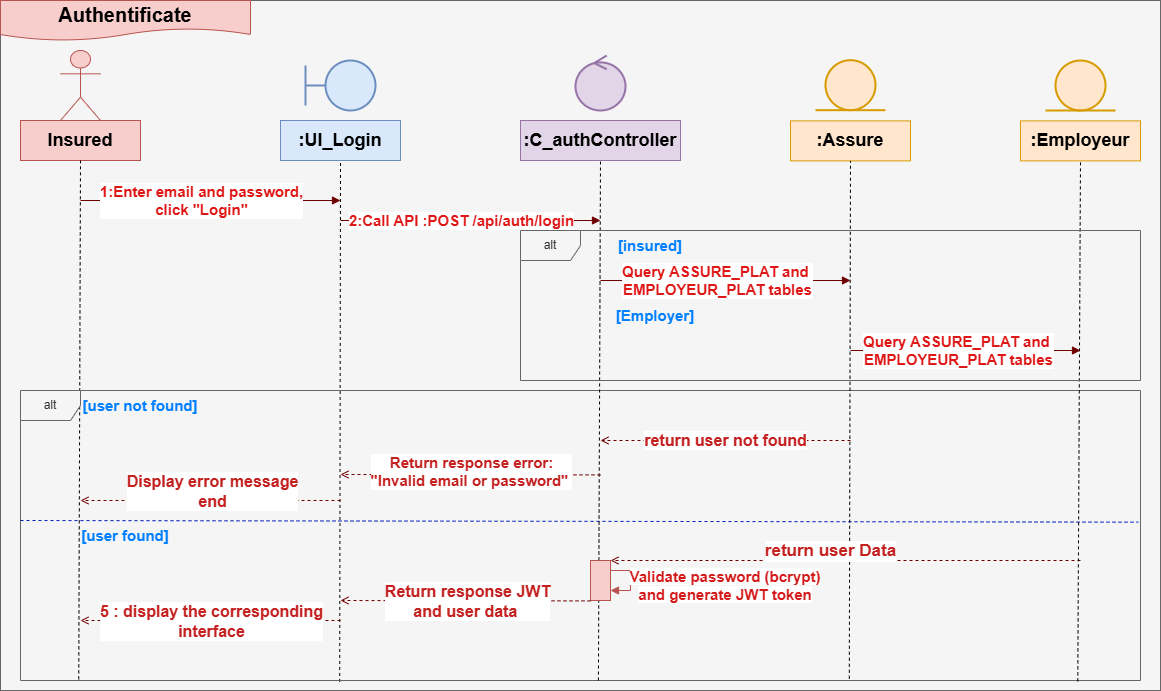
\includegraphics[width=1\textwidth]{figures/det authentificate.png}
    \caption{Detailed sequence diagram of the 'Authenticate' use case}
\end{figure}

\subsubsection{Detailed sequence diagram of the 'submit a service request' use case}
\begin{figure}[h!]
    \centering
    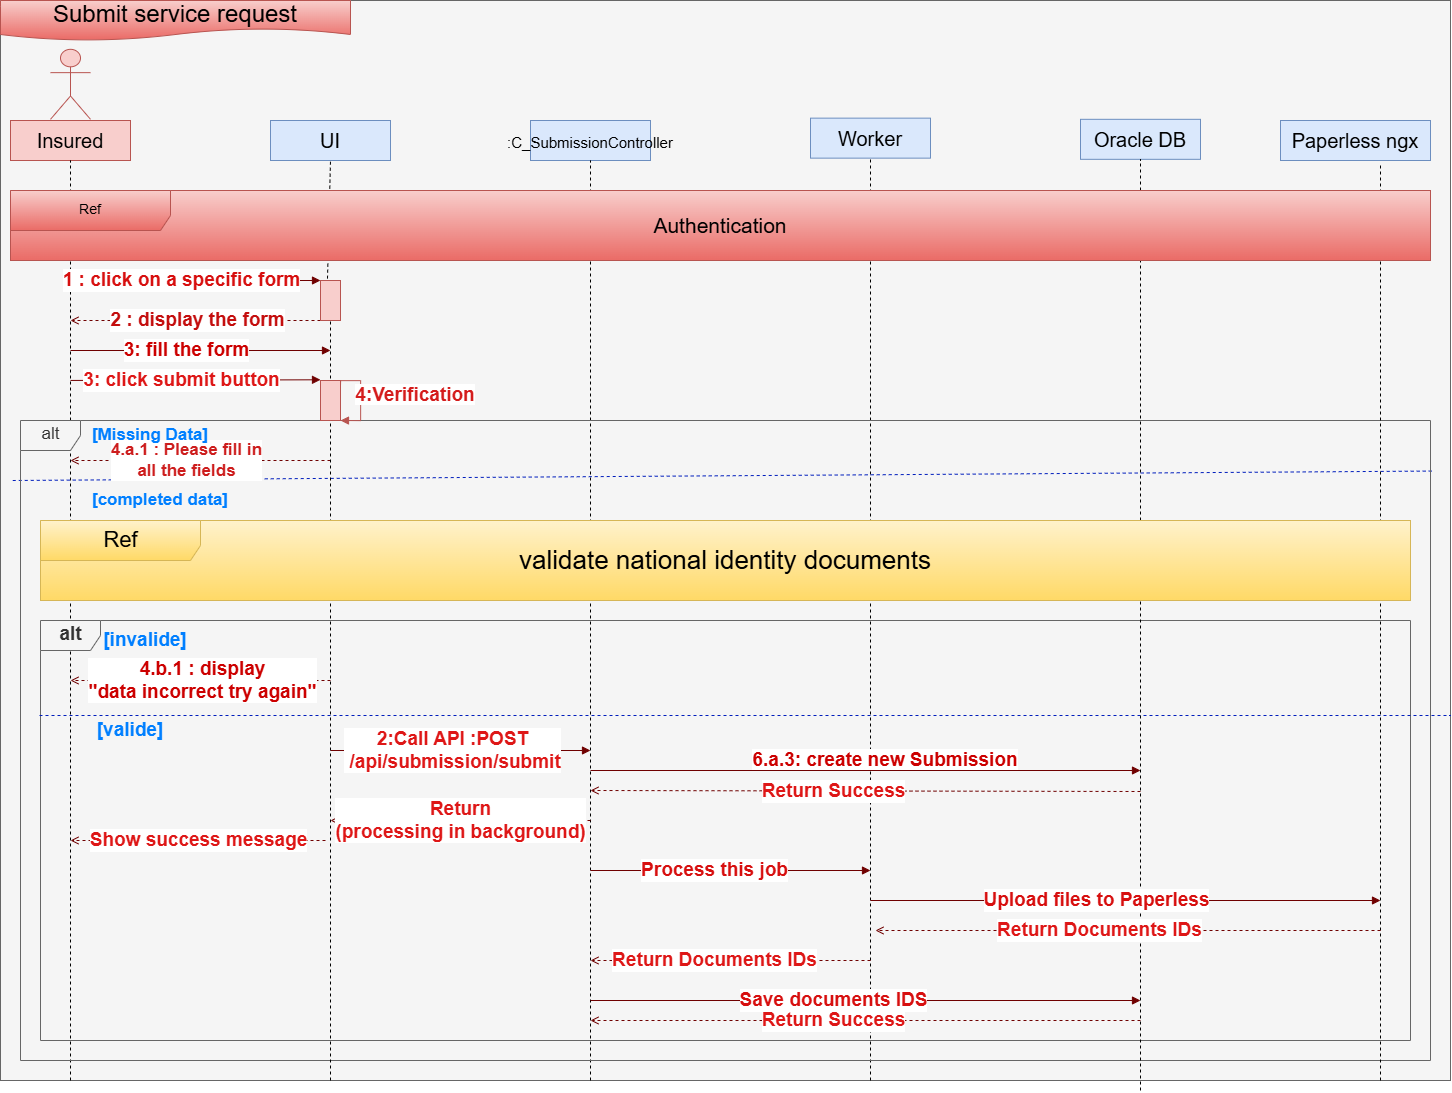
\includegraphics[width=1\textwidth]{figures/det Submits a service request.png}
    \caption{Detailed sequence diagram of the 'submit a service request' use case}
\end{figure}
\clearpage

\subsubsection{Detailed sequence diagram of the 'Manage Profile' use case}
\begin{figure}[h!]
    \centering
    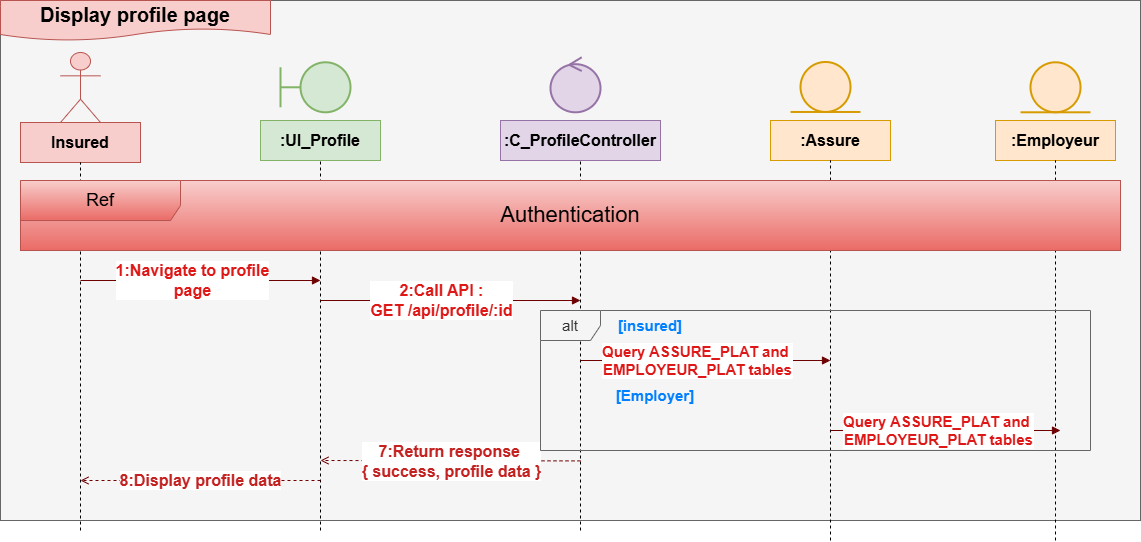
\includegraphics[width=1\textwidth]{figures/det display profile.png}
    \caption{Detailed sequence diagram of the 'Display Profile' use case}
\end{figure}
\begin{figure}[h!]
    \centering
    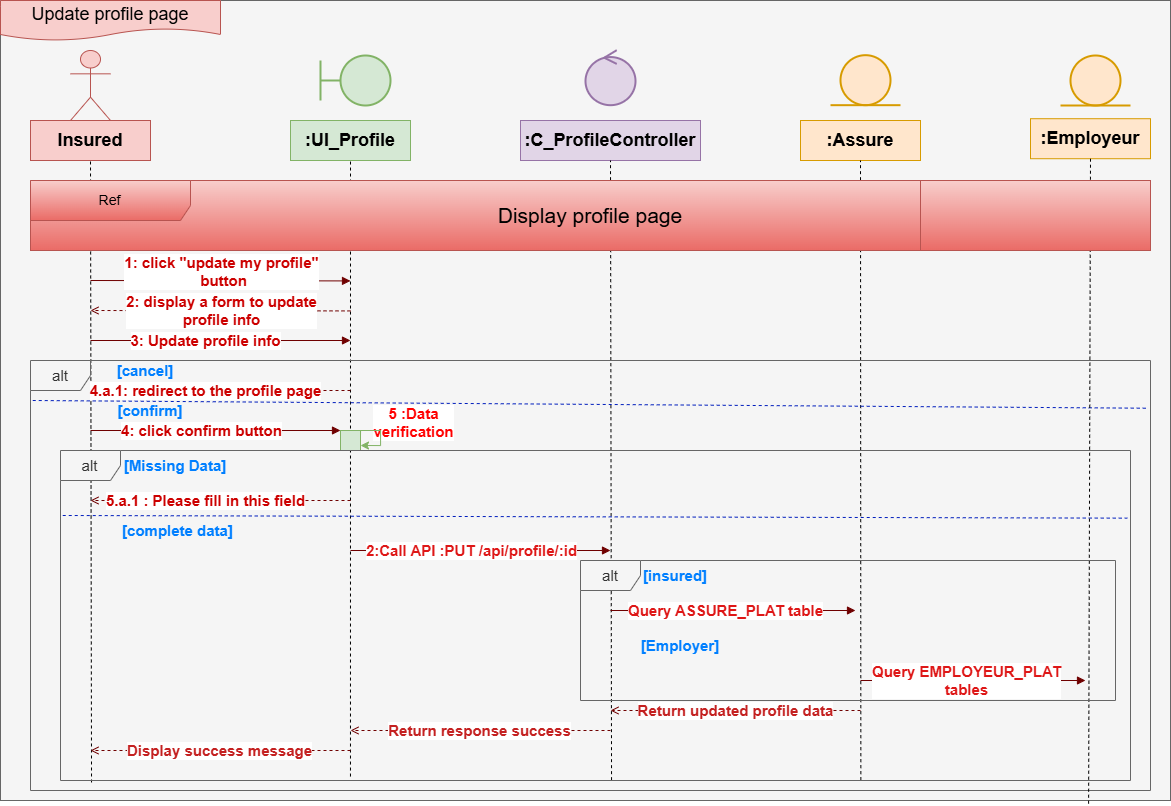
\includegraphics[width=1\textwidth]{figures/det update profile.png}
    \caption{Detailed sequence diagram of the 'Update Profile' use case}
\end{figure}
\clearpage
\begin{figure}[h!]
    \centering
    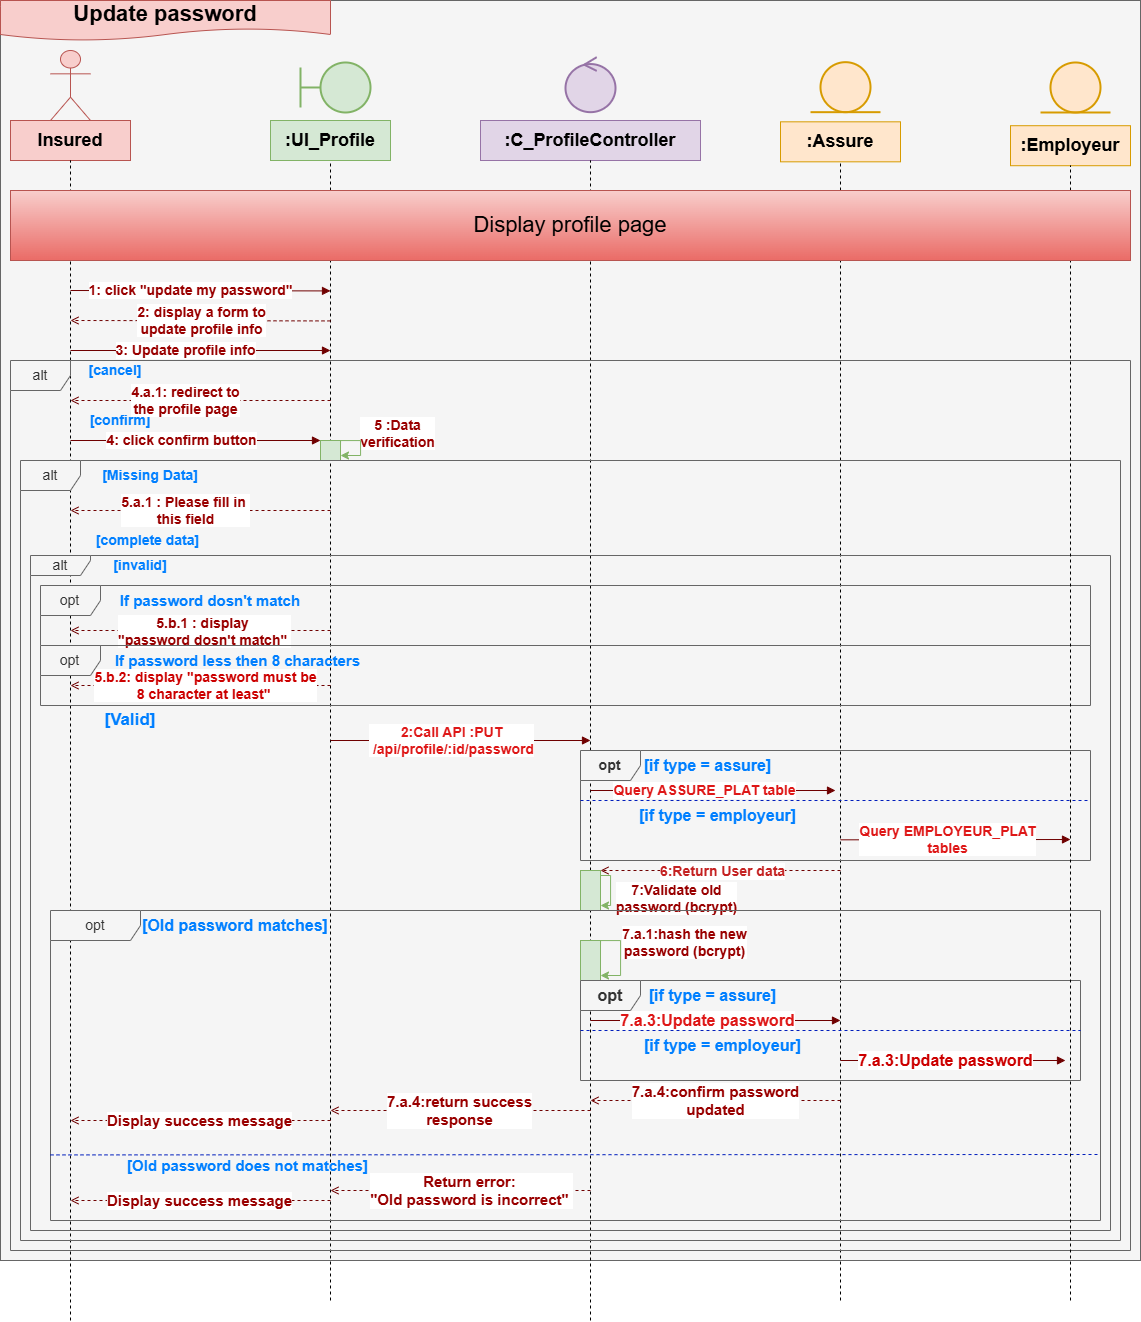
\includegraphics[width=1\textwidth]{figures/det update password.png}
    \caption{Detailed sequence diagram of the 'Update Password' use case}
\end{figure}
\clearpage
\subsubsection{Detailed sequence diagram of the 'Review Submission' use case}
\begin{figure}[h!]
    \centering
    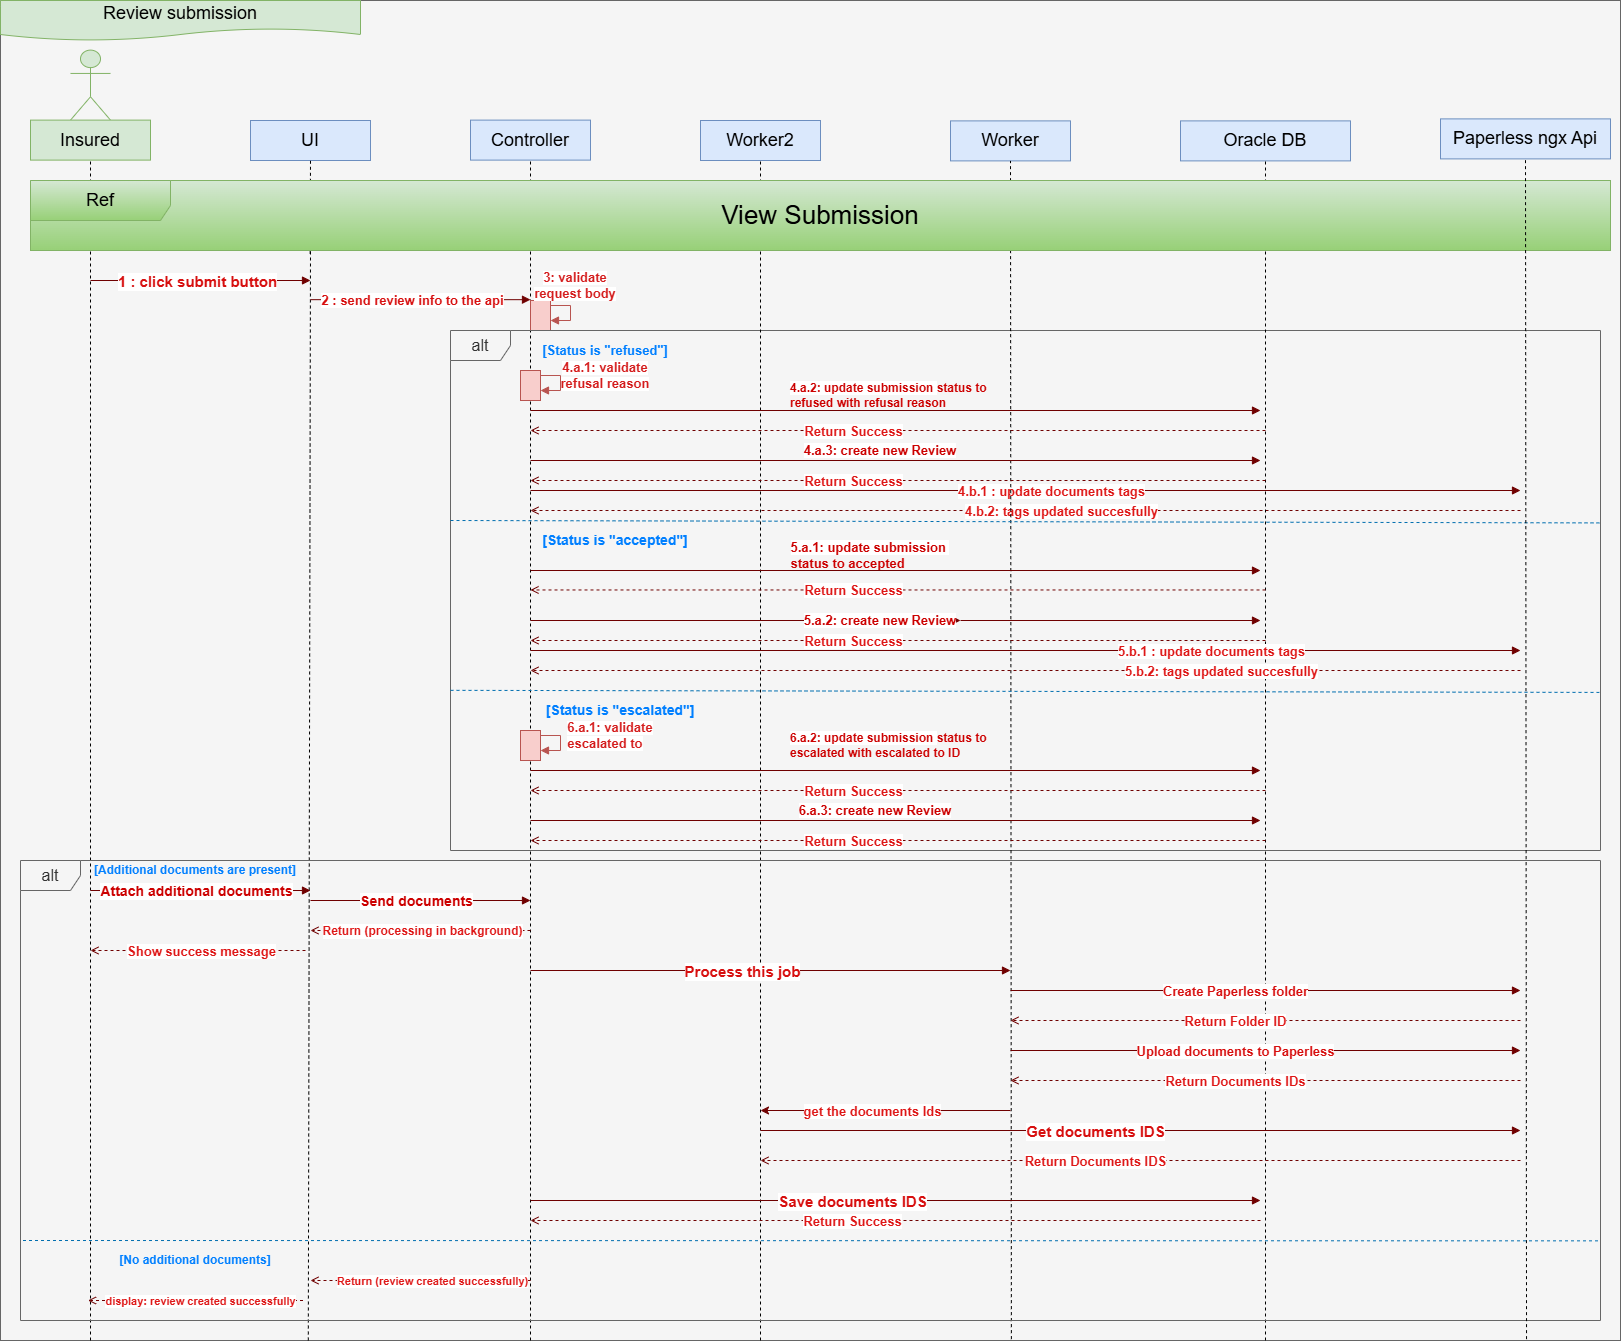
\includegraphics[width=1\textwidth]{figures/det review submission.png}
    \caption{Detailed sequence diagram of the 'Review Submission' use case}
\end{figure}
\clearpage
\subsubsection{Detailed sequence diagram of the 'Manage Internal stakeholders' use case}
\begin{figure}[h!]
    \centering
    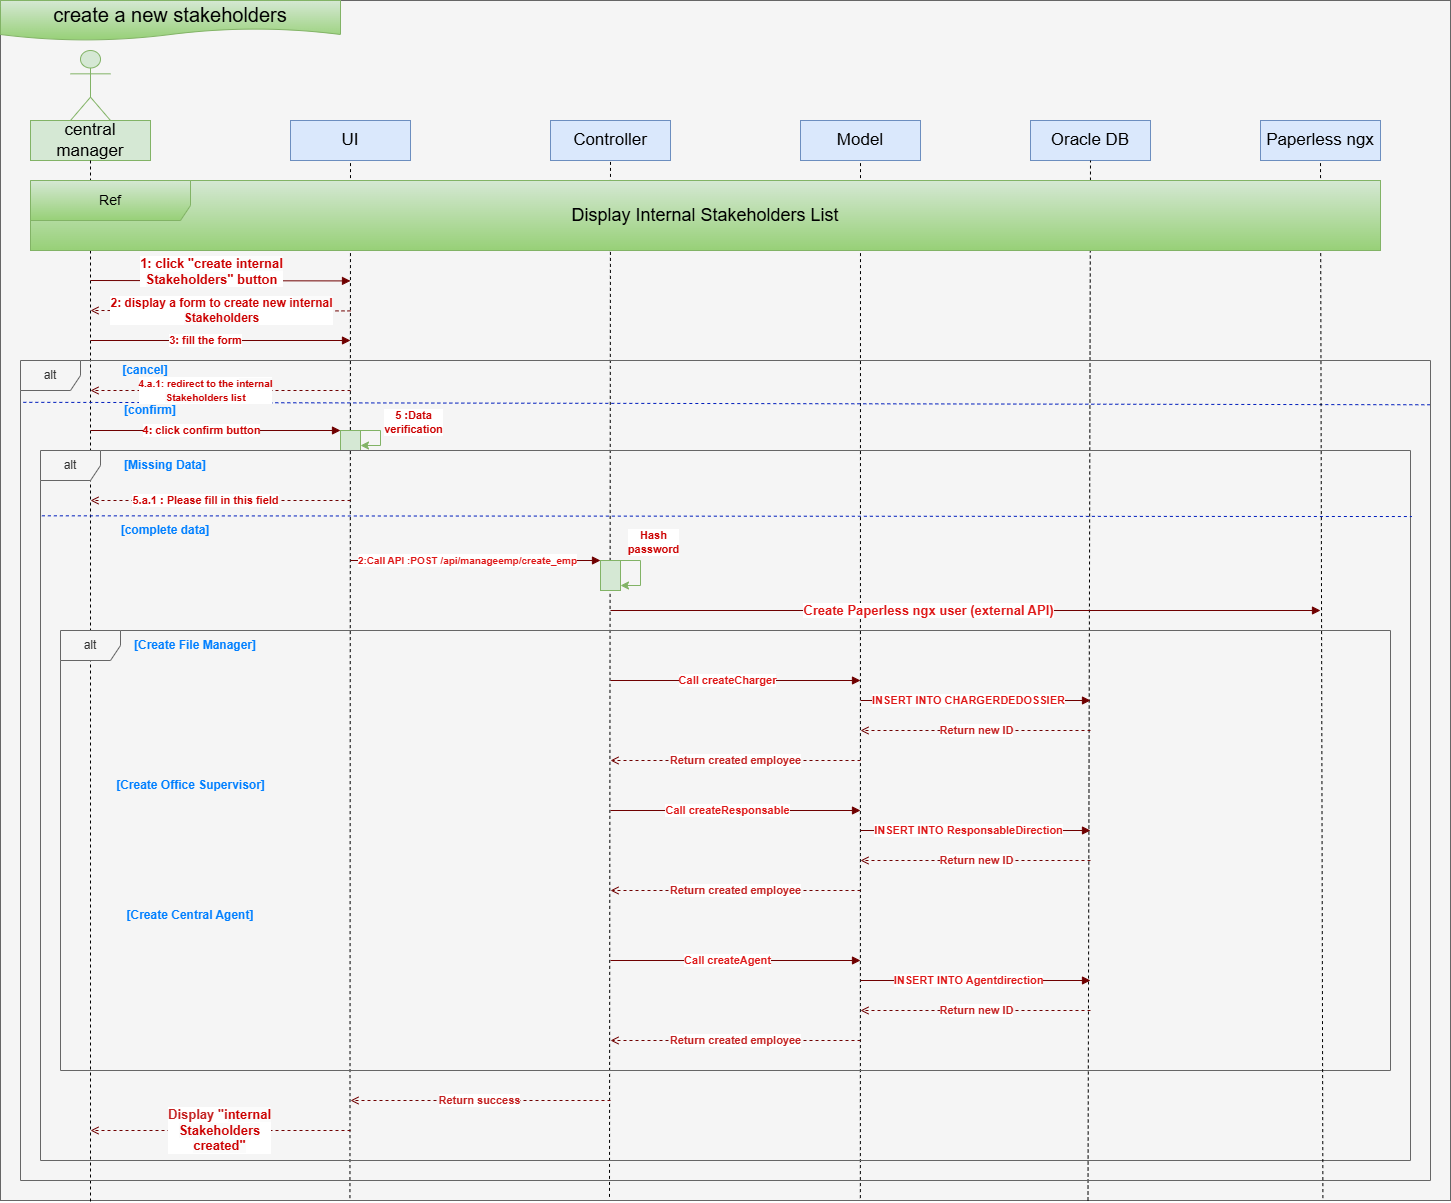
\includegraphics[width=1\textwidth]{figures/det Manages Internal Stakeholders create.png}
    \caption{Detailed sequence diagram of the 'Create a new stakeholder' use case}
    \label{fig:image4}
\end{figure}
\begin{figure}[h!]
    \centering
    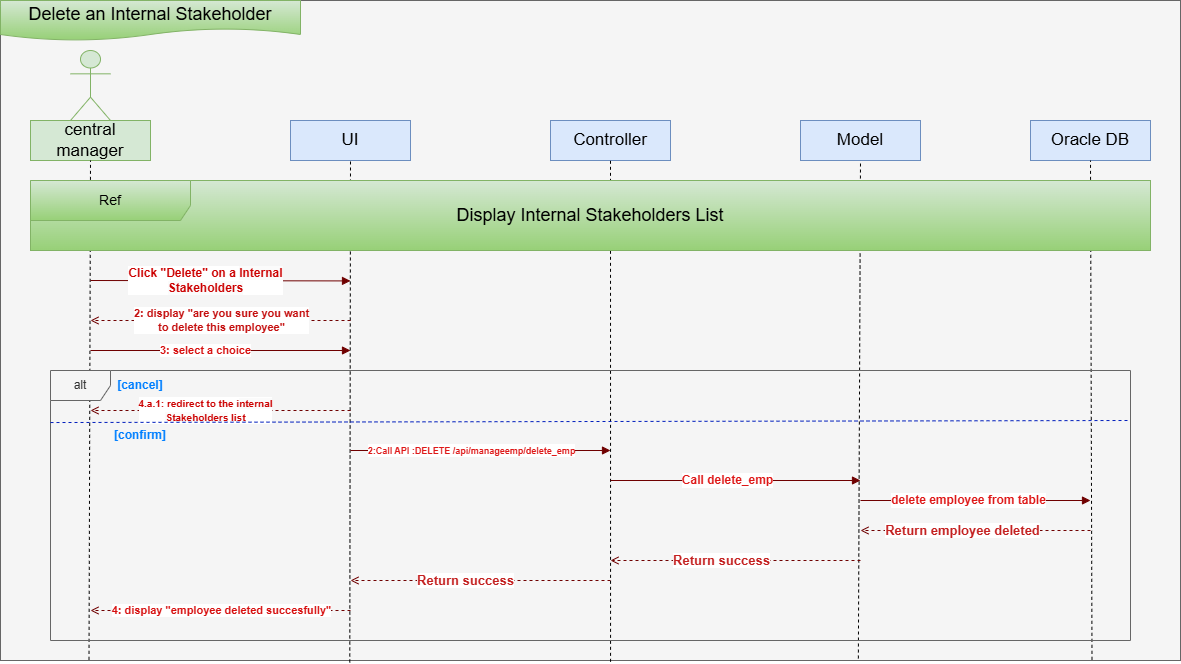
\includegraphics[width=1\textwidth]{figures/det Manages Internal Stakeholders delete.png}
    \caption{Detailed sequence diagram of the 'Delete a stakeholder' use case}
\end{figure}
\begin{figure}[h!]
    \centering
    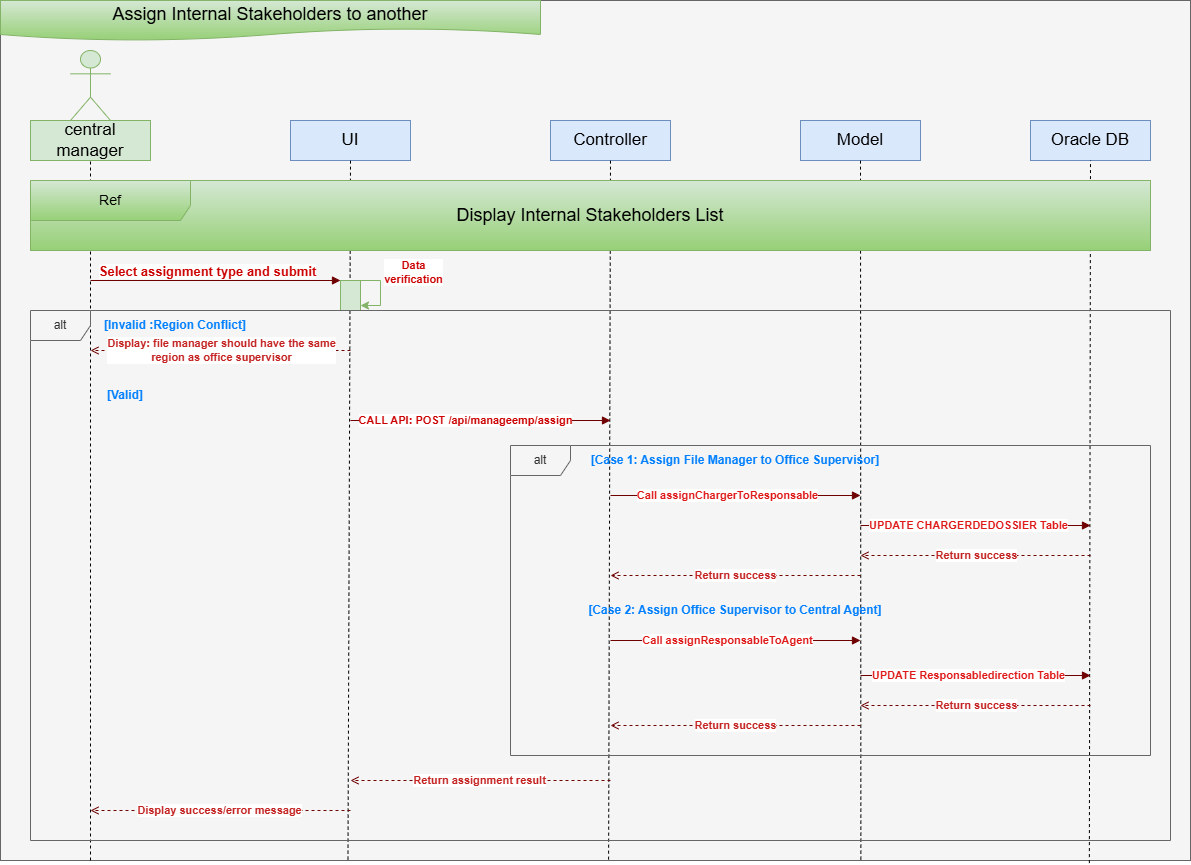
\includegraphics[width=1\textwidth]{figures/det Manages Internal Stakeholders assign.png}
    \caption{Detailed sequence diagram of the 'Assign a stakeholder' use case}
\end{figure}
\clearpage
\subsubsection{Detailed sequence diagram of the 'Manage Dynamic Forms' use case}
\begin{figure}[h!]
    \centering
    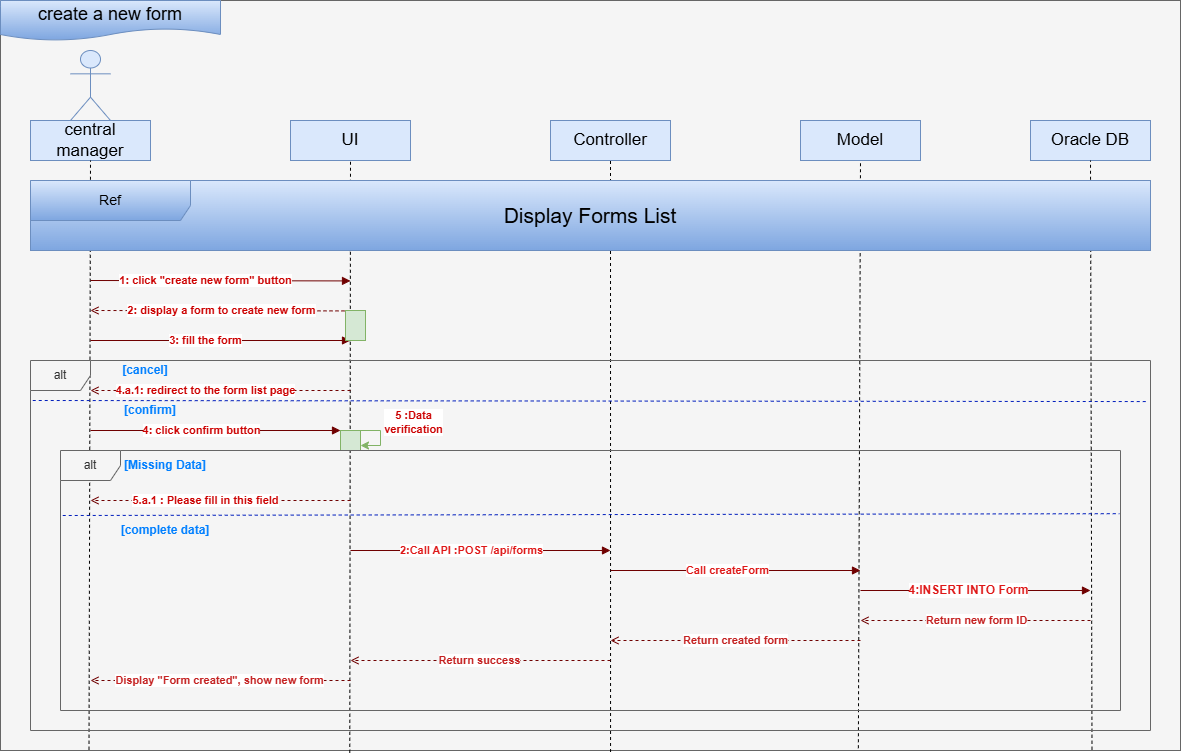
\includegraphics[width=1\textwidth]{figures/det manages dynamic form create a form.png}
    \caption{Detailed sequence diagram of the 'Create a form' use case}
\end{figure}
\begin{figure}[h!]
    \centering
    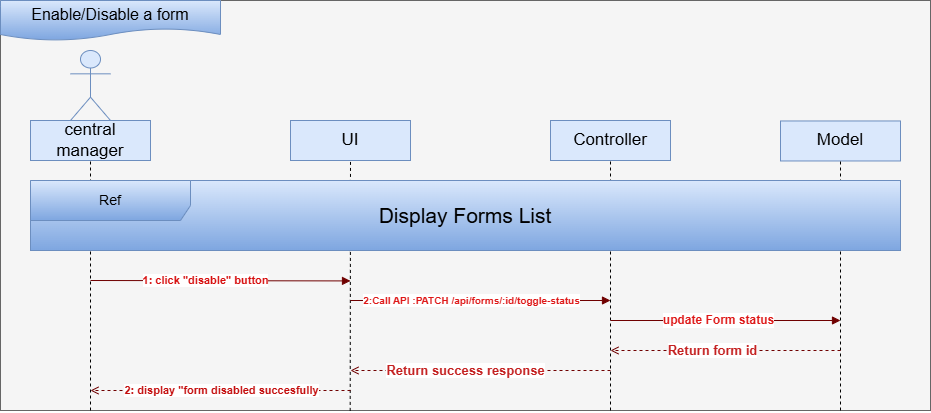
\includegraphics[width=1\textwidth]{figures/det enable a form.png}
    \caption{Detailed sequence diagram of the 'Disable/Enable a form' use case}
\end{figure}
\clearpage


\section{Global class diagram of the first sprint}
\begin{figure}[h!]
    \centering
    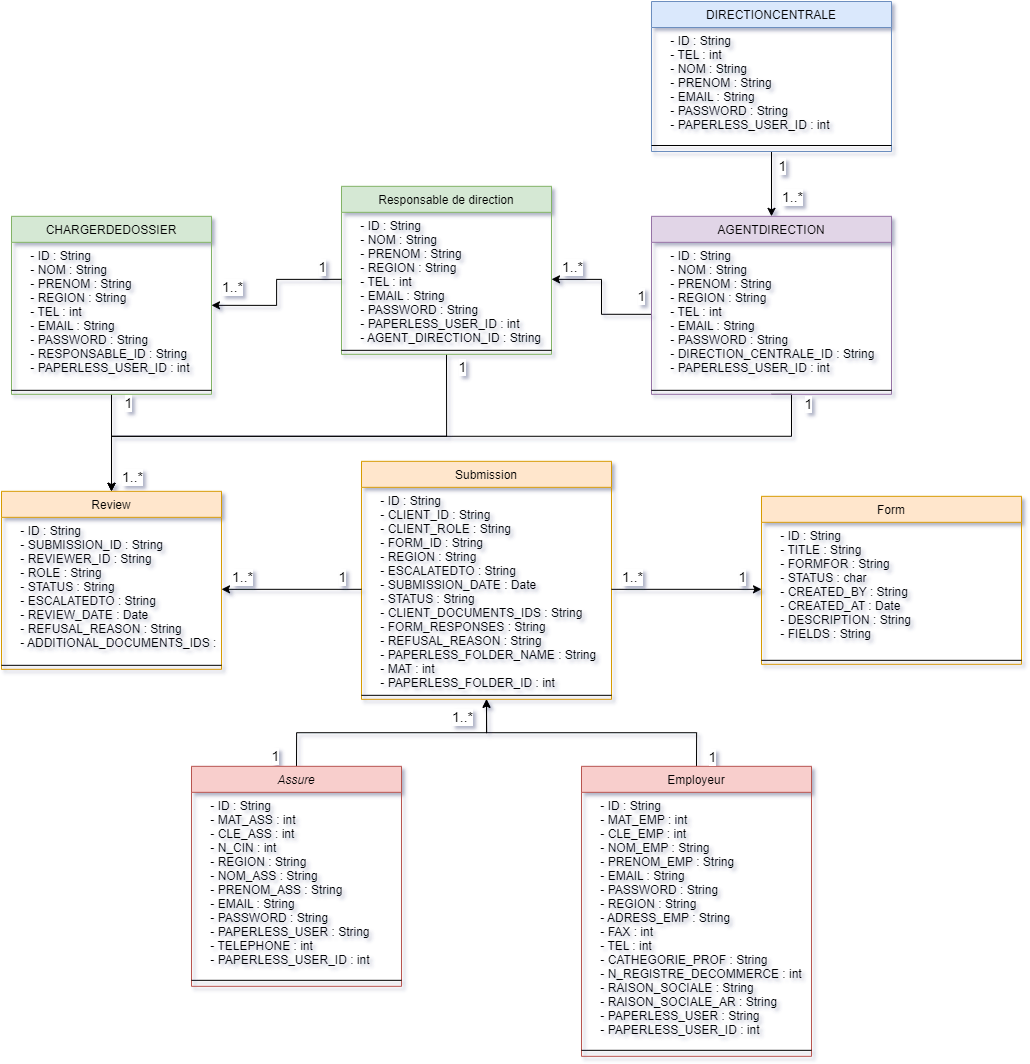
\includegraphics[width=1\textwidth]{figures/global_class_diagram_sprint_1-diagram_de_classe_sprint_1.png}
    \caption{Global class diagram of Sprint 1.}
\end{figure}
\clearpage
\section{Implementation}
The stage of implementation, or "coding", is dedicated to implementing the user stories contained within the first sprint.
In this case, we will establish the database structure for the current sprint using the rules to map the entity-association model into the relational model.
\begin{itemize}
    \item \textbf{Rule 1:} One entity is mapped onto a table (relation).
    \item \textbf{Rule 2:} A "one-to-many" relationship results in the shifting of the primary key from the parent table to the child table as a foreign key.
    \item \textbf{Rule 3:} A "many-to-many" relationship is represented by an extra table whose primary key consists of the primary keys of related tables.
\end{itemize}

\subsection{The Database Schemas}
\begin{table}[h!]
\centering
\begin{tabular}{|l|l|l|}
\hline
\textbf{Attribut} & \textbf{Type} & \textbf{Contrainte} \\
\hline
ID & VARCHAR & PRIMARY KEY \\
NOM & VARCHAR(50) & Not Null \\
PRENOM & VARCHAR(50) & Not Null \\
REGION & VARCHAR(50) & - \\
TEL & VARCHAR(15) & - \\
EMAIL & VARCHAR(100) & UNIQUE - Not Null \\
PASSWORD & VARCHAR(255) & Not Null \\
RESPONSABLE\_ID & VARCHAR & FOREIGN KEY - Not Null \\
PAPERLESS\_USER\_ID & INT & FOREIGN KEY - Not Null \\
\hline
\end{tabular}
\caption{Table \texttt{CHARGERDEDOSSIER}}
\end{table}
\begin{table}[h!]
\centering
\begin{tabular}{|l|l|l|}
\hline
\textbf{Attribut} & \textbf{Type} & \textbf{Contrainte} \\
\hline
ID & VARCHAR & PRIMARY KEY \\
NOM & VARCHAR(50) & Not Null \\
PRENOM & VARCHAR(50) & Not Null \\
REGION & VARCHAR(50) & - \\
TEL & VARCHAR(15) & - \\
EMAIL & VARCHAR(100) & UNIQUE - Not Null \\
PASSWORD & VARCHAR(255) & Not Null \\
PAPERLESS\_USER\_ID & INT & FOREIGN KEY - Not Null \\
AGENT\_DIRECTION\_ID & VARCHAR & FOREIGN KEY \\
\hline
\end{tabular}
\caption{Table \texttt{ResponsableDirection}}
\end{table}
\begin{table}[h!]
\centering
\begin{tabular}{|l|l|l|}
\hline
\textbf{Attribut} & \textbf{Type} & \textbf{Contrainte} \\
\hline
ID & VARCHAR & PRIMARY KEY \\
NOM & VARCHAR(50) & Not Null \\
PRENOM & VARCHAR(50) & Not Null \\
REGION & VARCHAR(50) & - \\
TEL & VARCHAR(15) & - \\
EMAIL & VARCHAR(100) & UNIQUE - Not Null \\
PASSWORD & VARCHAR(255) & Not Null \\
DIRECTION\_CENTRALE\_ID & VARCHAR & FOREIGN KEY \\
PAPERLESS\_USER\_ID & INT & FOREIGN KEY - Not Null \\
\hline
\end{tabular}
\caption{Table \texttt{AgentDirection}}
\end{table}
\begin{table}[h!]
\centering
\begin{tabular}{|l|l|l|}
\hline
\textbf{Attribut} & \textbf{Type} & \textbf{Contrainte} \\
\hline
ID & VARCHAR & PRIMARY KEY \\
TEL & INT & - \\
NOM & VARCHAR(50) & Not Null \\
PRENOM & VARCHAR(50) & Not Null \\
EMAIL & VARCHAR(100) & UNIQUE - Not Null \\
PASSWORD & VARCHAR(255) & Not Null \\
PAPERLESS\_USER\_ID & INT & FOREIGN KEY - Not Null \\
\hline
\end{tabular}
\caption{Table \texttt{DirectionCentrale}}
\end{table}
\begin{table}[h!]
\centering
\begin{tabular}{|l|l|l|}
\hline
\textbf{Attribut} & \textbf{Type} & \textbf{Contrainte} \\
\hline
ID & VARCHAR & PRIMARY KEY \\
CLIENT\_ID & VARCHAR & FOREIGN KEY \\
CLIENT\_ROLE & VARCHAR(50) & Not Null \\
FORM\_ID & VARCHAR & FOREIGN KEY \\
REGION & VARCHAR(50) & - \\
ESCALATEDTO & VARCHAR & - \\
SUBMISSION\_DATE & DATE & Not Null \\
STATUS & VARCHAR(20) & Not Null \\
CLIENT\_DOCUMENTS\_IDS & VARCHAR(255) & - \\
FORM\_RESPONSES & TEXT & - \\
REFUSAL\_REASON & TEXT & - \\
PAPERLESS\_FOLDER\_NAME & VARCHAR(255) & - \\
MAT & INT & - \\
PAPERLESS\_FOLDER\_ID & INT & FOREIGN KEY - Not Null \\
\hline
\end{tabular}
\caption{Table \texttt{Submission}}
\end{table}

\begin{table}[h!]
\centering
\begin{tabular}{|l|l|l|}
\hline
\textbf{Attribut} & \textbf{Type} & \textbf{Contrainte} \\
\hline
ID & VARCHAR & PRIMARY KEY \\
TITLE & VARCHAR(255) & Not Null \\
FORM\_FOR & VARCHAR(50) & - \\
STATUS & CHAR(1) & Not Null \\
CREATED\_BY & VARCHAR(50) & - \\
CREATED\_AT & DATE & Not Null \\
DESCRIPTION & TEXT & - \\
FIELDS & TEXT & - \\
\hline
\end{tabular}
\caption{Table \texttt{Form}}
\end{table}
\begin{table}[h!]
\centering
\begin{tabular}{|l|l|l|}
\hline
\textbf{Attribut} & \textbf{Type} & \textbf{Contrainte} \\
\hline
ID & VARCHAR & PRIMARY KEY \\
SUBMISSION\_ID & VARCHAR & FOREIGN KEY \\
REVIEWER\_ID & VARCHAR & FOREIGN KEY \\
ROLE & VARCHAR(50) & - \\
STATUS & VARCHAR(50) & - \\
ESCALATEDTO & VARCHAR & - \\
REVIEW\_DATE & DATE & - \\
REFUSAL\_REASON & TEXT & - \\
ADDITIONAL\_DOCUMENTS\_IDS & TEXT & - \\
\hline
\end{tabular}
\caption{Table \texttt{Review}}
\end{table}

\begin{table}[h!]
\centering
\begin{tabular}{|l|l|l|}
\hline
\textbf{Attribut} & \textbf{Type} & \textbf{Contrainte} \\
\hline
ID & VARCHAR & PRIMARY KEY \\
MAT\_ASS & INT & UNIQUE - Not Null \\
CLE\_ASS & INT & - \\
REGION & VARCHAR(50) & - \\
NOM\_ASS & VARCHAR(50) & Not Null \\
PRENOM\_ASS & VARCHAR(50) & Not Null \\
EMAIL & VARCHAR(100) & UNIQUE - Not Null \\
PASSWORD & VARCHAR(255) & Not Null \\
PAPERLESS\_USER\_ID & INT & FOREIGN KEY - Not Null \\
TELEPHONE & INT & - \\
\hline
\end{tabular}
\caption{Table \texttt{Assure}}
\end{table}
\begin{table}[h!]
\centering
\begin{tabular}{|l|l|l|}
\hline
\textbf{Attribut} & \textbf{Type} & \textbf{Contrainte} \\
\hline
ID & VARCHAR & PRIMARY KEY \\
MAT\_EMP & INT & UNIQUE - Not Null \\
CLE\_EMP & INT & - \\
NOM\_EMP & VARCHAR(50) & Not Null \\
PRENOM\_EMP & VARCHAR(50) & Not Null \\
EMAIL & VARCHAR(100) & UNIQUE - Not Null \\
PASSWORD & VARCHAR(255) & Not Null \\
REGION & VARCHAR(50) & - \\
ADRESSE\_EMP & TEXT & - \\
FAX & INT & - \\
TEL & INT & - \\
CATEGORIE\_PROF & VARCHAR(50) & - \\
N\_REGISTRE\_DECOMMERCE & VARCHAR(50) & - \\
RAISON\_SOCIALE & VARCHAR(255) & - \\
RAISON\_SOCIALE\_AR & VARCHAR(255) & - \\
PAPERLESS\_USER\_ID & INT & FOREIGN KEY - Not Null \\
\hline
\end{tabular}
\caption{Table \texttt{Employeur}}
\end{table}
\clearpage
\subsection{The interfaces of the use cases}
\begin{figure}[h!]
    \centering
    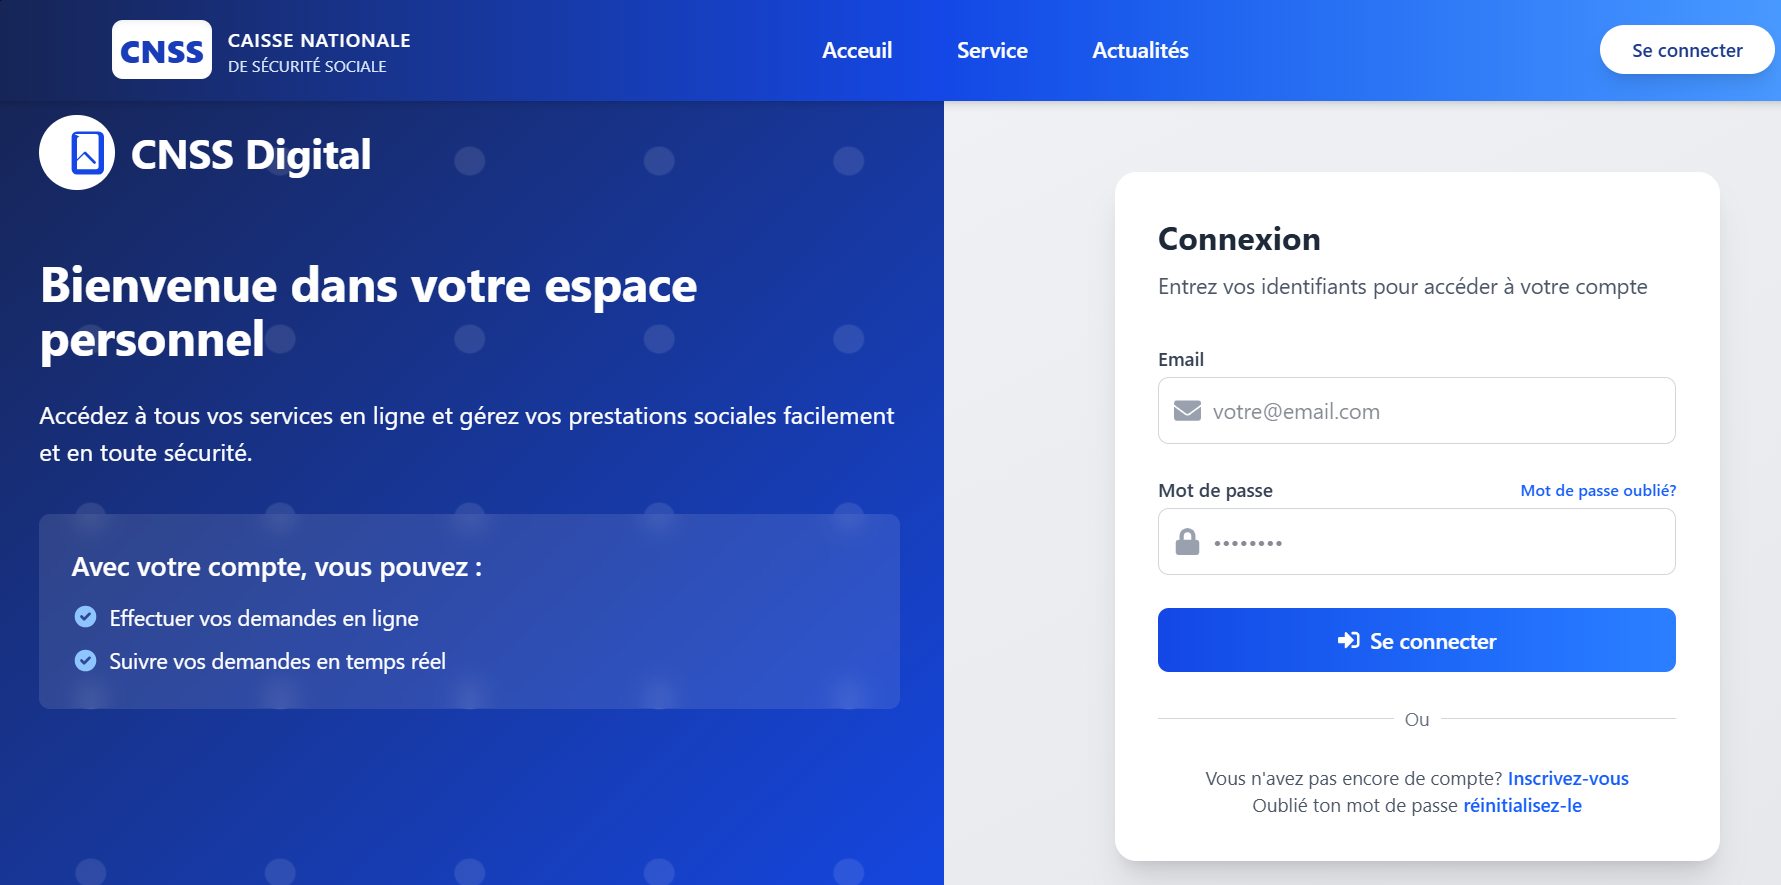
\includegraphics[width=1\textwidth]{figures/ui-auth.png}
    \caption{Interface of the Login page.}
\end{figure}
\begin{figure}[h!]
    \centering
    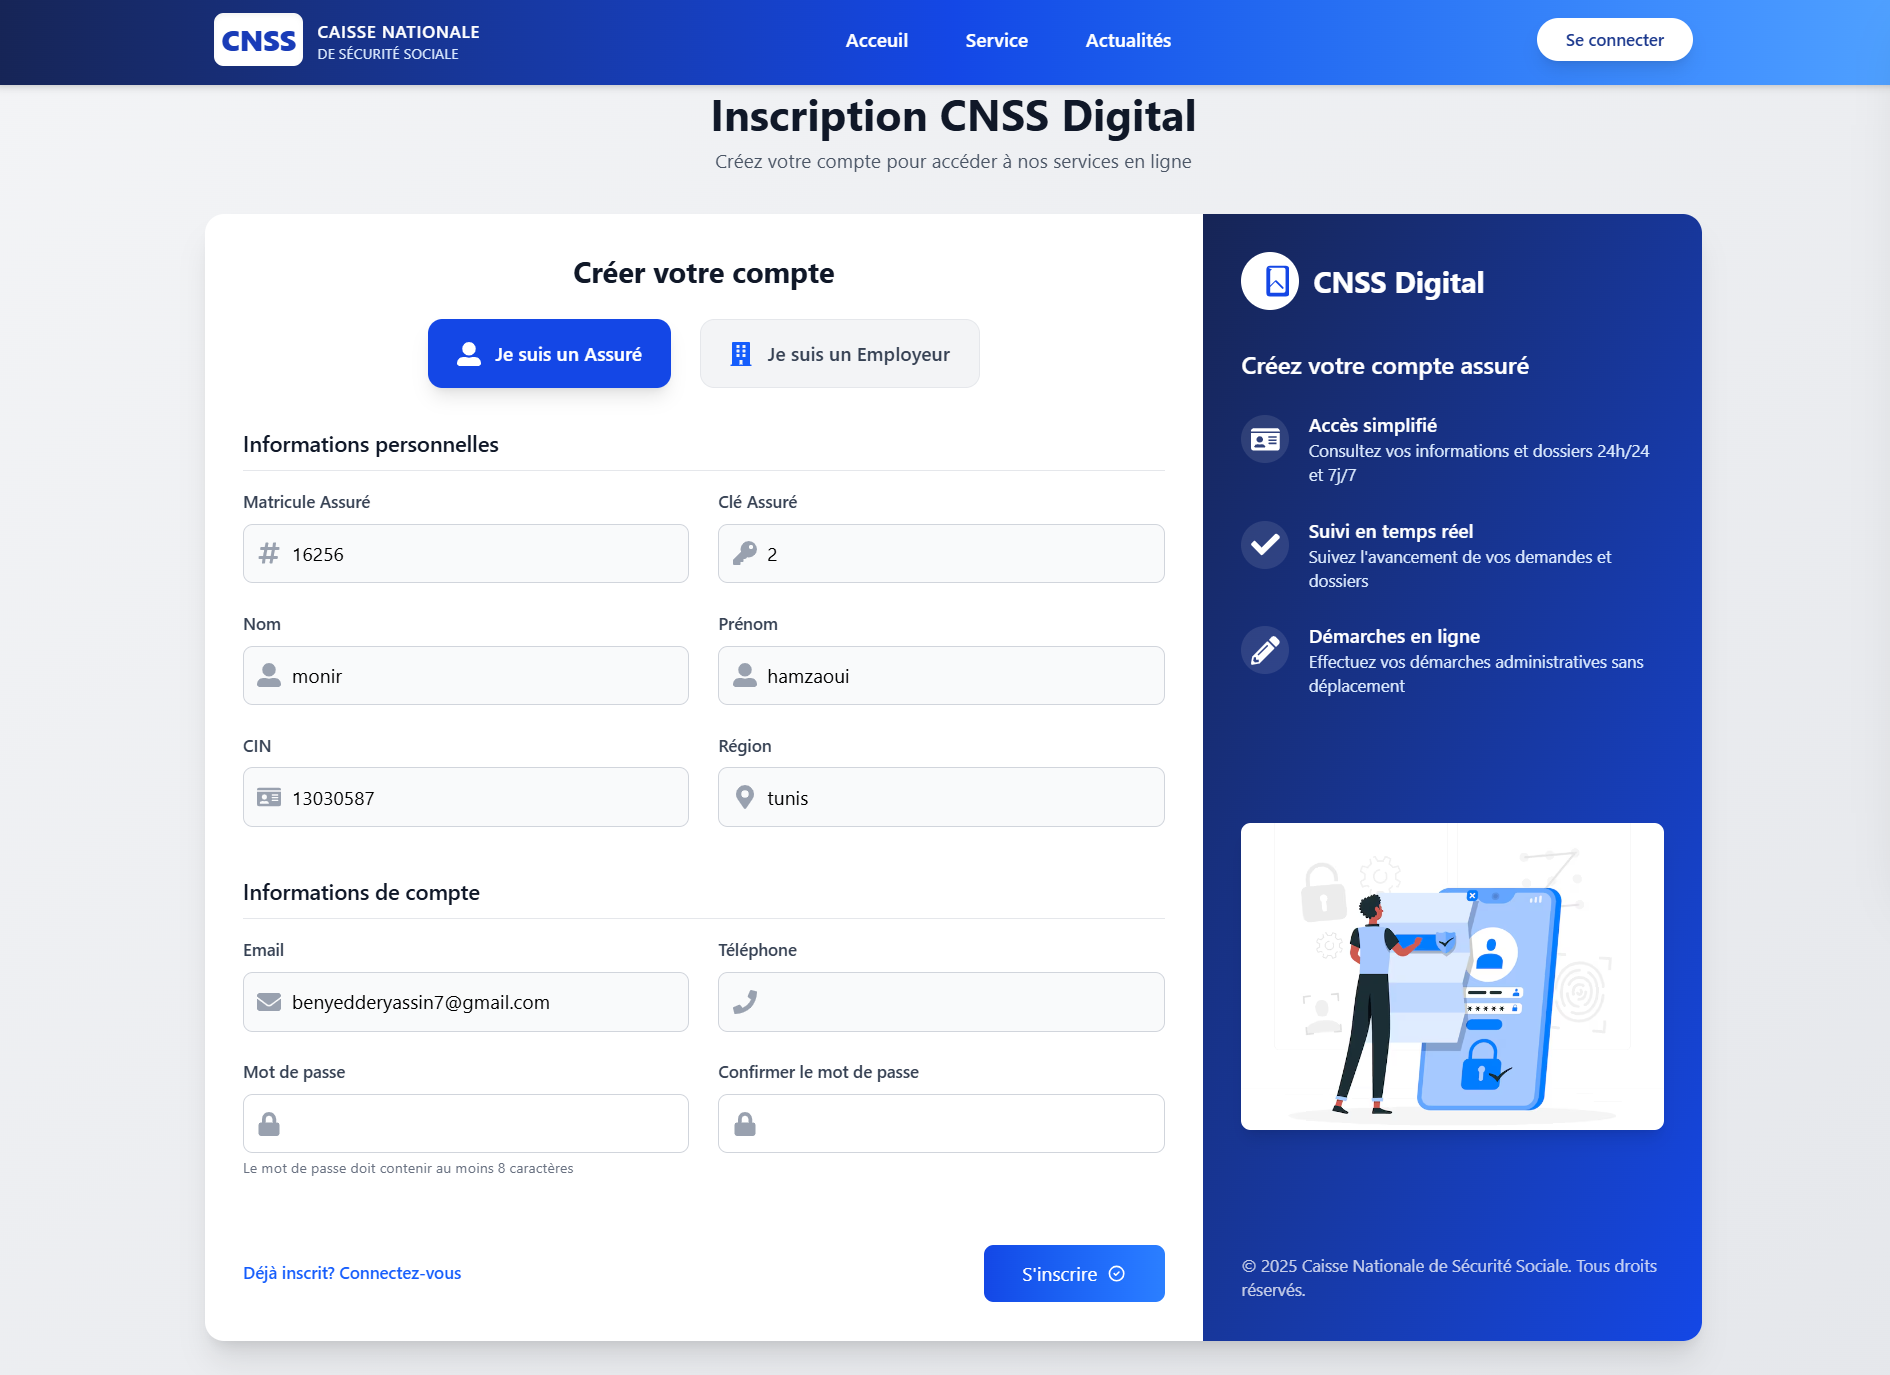
\includegraphics[width=1\textwidth]{figures/ui-signup.png}
    \caption{Interface of the Sign-up page.}
\end{figure}

\begin{figure}[h!]
    \centering
    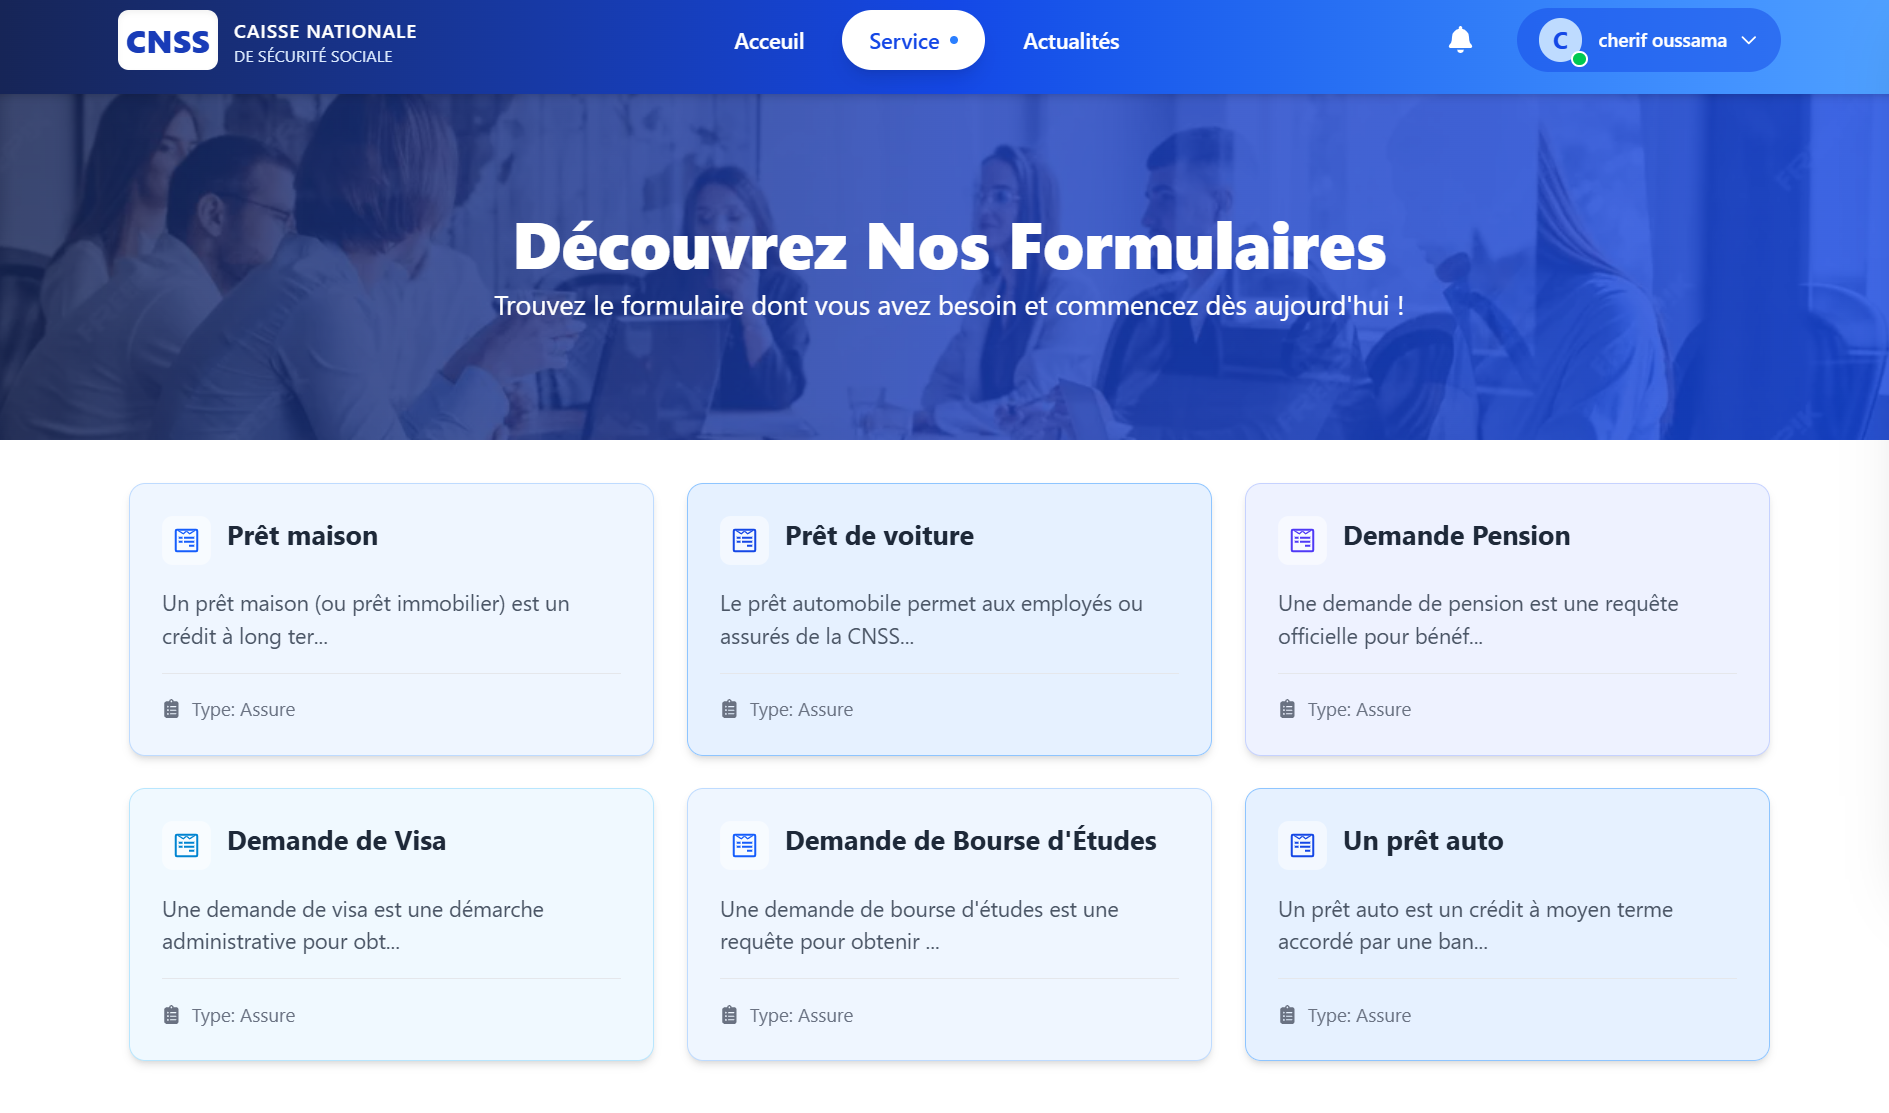
\includegraphics[width=1\textwidth]{figures/ui-servicepage.png}
    \caption{Interface of the Service page.}
\end{figure}
\begin{figure}[h!]
    \centering
    \includegraphics[width=1\textwidth]{figures/ui-detform.png}
    \caption{Interface of the Form details page.}
\end{figure}
\begin{figure}[h!]
    \centering
    \includegraphics[width=1\textwidth]{figures/ui-form.png}
    \caption{Interface of the Form page.}
\end{figure}
\begin{figure}[h!]
    \centering
    \includegraphics[width=1\textwidth]{figures/ui-reviewsub.png}
    \caption{Interface of the Review Submissions page.}
\end{figure}
\begin{figure}[h!]
    \centering
    \includegraphics[width=1\textwidth]{figures/ui-reviewsubdetails.png}
    \caption{Interface of the Review Submissions details page.}
\end{figure}
\begin{figure}[h!]
    \centering
    \includegraphics[width=1\textwidth]{figures/ui-profile.png}
    \caption{Interface of the Profile page.}
\end{figure}
\begin{figure}[h!]
    \centering
    \includegraphics[width=1\textwidth]{figures/ui-managestakeholders.png}
    \caption{Interface of the Manage Internal stakeholders page.}
\end{figure}
\begin{figure}[h!]
    \centering
    \includegraphics[width=1\textwidth]{figures/ui-manageform.png}
    \caption{Interface of Manage Form page.}
\end{figure}
\begin{figure}[h!]
    \centering
    \includegraphics[width=1\textwidth]{figures/ui-createform.png}
    \caption{Interface of create a form page.}
\end{figure}
\clearpage
\section{Tests}
\textbf{\textit{"The role of testing in the agile method is essential for the proper execution of developments. In order to ensure the reliability of the developed functionalities, it is unthinkable to pass through the sprints without having tested them beforehand: tests therefore play a crucial role."\cite{samplewebs7}}}
\subsection{Unit Tests}
We continue to work with the open source Jest unit testing framework to demonstrate in this section some examples of unit tests performed, along with the reasoning behind their implementation.
\subsection{ Unit Test for the Use Case "Submit a service request"}
\subsubsection{Reasoning} 
To test the submission of the file, we followed this reasoning:\\  
\begin{itemize}
    \item Creation of a form object.  
   \item Input of information related to the object's attributes.  
\item Insertion of the form into the database and the documents into the GED.  
\item Testing whether the form was successfully submitted.
\end{itemize}
\subsubsection{Successful Test Case "Submit a service request"} 
In the case of success, the test performed should return a positive result.
\begin{figure}[h!]
    \centering
    \includegraphics[width=1\textwidth]{figures/subScode.JPG}  % Replace with your image file
    \caption{Source code of the method submit a service request.}
\end{figure} \
\begin{figure}[h!]
    \centering
    \includegraphics[width=1\textwidth]{figures/test success submit service request.png}  
    \caption{Result of the test submitting a file request.}
\end{figure} \
\clearpage
\subsubsection{Failure Test Case "Submit a service request"}
In the case of a fail, the test performed should return a negative result.
\begin{figure}[h!]
    \centering
    \includegraphics[width=1\textwidth]{figures/subFcode.JPG}
    \caption{Source code of the method submit a service request.}
\end{figure} \
\begin{figure}[h!]
    \centering
    \includegraphics[width=1\textwidth]{figures/test fail submit service request.png}  
    \caption{Result of the test submitting a file request.}
\end{figure} \



\subsection{ Unit Test for the Use Case "Create Dynamic forms"}
\subsubsection{Reasoning} 
To test the creation of a new form, we followed this reasoning:\\  
\begin{itemize}
    \item Creation of a form object.  
   \item Input of information related to the object's attributes.  
\item Insertion of the form into the database.  
\item Testing whether the form was successfully created.
\end{itemize}
\subsubsection{Successful Test Case "Create a dynamic form"} 
In the case of success, the test performed should return a positive result.
\begin{figure}[h!]
    \centering
    \includegraphics[width=1\textwidth]{figures/createformScode.JPG}
    \caption{Source code of the method create a form.}
\end{figure} \
\clearpage
\begin{figure}[h!]
    \centering
    \includegraphics[width=1\textwidth]{figures/test succes create form.png} 
    \caption{Result of the test creating a new form.}
\end{figure} \

\subsubsection{Failure Test Case "Submit a service request"}
In the case of a fail, the test performed should return a negative result.
\begin{figure}[h!]
    \centering
    \includegraphics[width=1\textwidth]{figures/createformFcode.JPG}
    \caption{Source code of the method create a new form.}
\end{figure} \
\begin{figure}[h!]
    \centering
    \includegraphics[width=1\textwidth]{figures/test fail create form.png}  % Replace with your image file
    \caption{Result of the test creating a new form.}
\end{figure} \
\section{Sprint Review – Burndown Chart Diagram}
\textbf{\textit{"A Burndown Chart is a simple graph that shows the progress in completing tasks. In other words, it is a graphical representation of how the amount of remaining work evolves over time, within a given period."\cite{samplewebs8}}}
\begin{table}[h!]
\centering
\small
\resizebox{\textwidth}{!}{%
\begin{tabular}{|c|c|c|c|c|c|}
\hline
\textbf{DAY} & \textbf{Hours Planned} & \textbf{Hours Actual} & \textbf{Remaining Planned} & \textbf{Remaining Actual} & \textbf{Done Today} \\
\hline
0 & -  & -  & 160 & 160 & -  \\
1 & 8  & 4  & 152 & 156 &    \\
2 & 8  & 6  & 144 & 149 & 7  \\
3 & 8  & 7  & 136 & 143 & 6  \\
4 & 8  & 6  & 128 & 134 & 9  \\
5 & 8  & 7  & 120 & 133 & 1  \\
6 & 8  & 10 & 112 & 126 & 7  \\
7 & 8  & 12 & 104 & 109 & 17 \\
8 & 8  & 8  & 96  & 102 & 7  \\
9 & 8  & 6  & 88  & 90  & 12 \\
10 & 8 & 0  & 80  & 90  & 0  \\
11 & 8 & 10 & 72  & 80  & 10 \\
12 & 8 & 8  & 64  & 67  & 13 \\
13 & 8 & 8  & 56  & 60  & 7  \\
14 & 8 & 7  & 48  & 47  & 13 \\
15 & 8 & 6  & 40  & 37  & 10 \\
16 & 8 & 7  & 32  & 30  & 7  \\
17 & 8 & 6  & 24  & 25  & 5  \\
18 & 8 & 8  & 16  & 16  & 9  \\
19 & 8 & 12 & 8   & 6   & 10 \\
20 & 8 & 8  & 0   & 0   & 6  \\
\hline
\end{tabular}%
}
\caption{Burndown Chart Table for Sprint 1 (20 Days)}
\end{table}
\begin{figure}[h!]
    \centering
    \includegraphics[width=0.7\textwidth]{figures/burn down chart 1.png} 
    \caption{Burn down chart of sprint 1.}
\end{figure} \
\newpage
\begin{center}
    \doublespacing  % Increase line spacing to double spacing
    \centering
    \LARGE\textbf{Conclusion} 
    \vspace{1cm} \\
    \raggedright
\end{center}
\addcontentsline{toc}{section}{Conclusion}
In this chapter, we focused on the development of our first sprint. As a result, we now have a potentially deliverable increment of our platform.
In the next chapter, we will focus on the implementation of our second sprint.













 -








